\documentclass[a4paper]{article}

% Basic packages
\usepackage{fontspec}
\XeTeXlinebreaklocale "zh"    % 启用中文断行（XeTeX 内建，无需 xeCJK）
\XeTeXlinebreakskip = 0pt plus 1pt
\setmainfont{Songti SC}
\setsansfont{Heiti SC}
\setmonofont{Menlo}
\usepackage{amsmath, amssymb}
\usepackage{graphicx}
\usepackage[margin=2.5cm]{geometry}
\usepackage[most]{tcolorbox}
\usepackage{etoolbox}
\usepackage{listings}
\usepackage{hyperref}
\usepackage{booktabs}
\usepackage{subcaption}
\usepackage{float}

% Chinese font setup (macOS system fonts, no ctex needed)
\setmainfont{Songti SC}
\setsansfont{Heiti SC}
\setmonofont{Menlo}
\newcommand{\song}{\fontspec{Songti SC}}
\newcommand{\hei}{\fontspec{Heiti SC}}
\newcommand{\kai}{\fontspec{KaiTi}}
\newcommand{\fangsong}{\fontspec{FangSong}}

% ===== Highlight boxes =====
\newtcolorbox{knowledgebox}[1]{
    enhanced, colback=blue!5!white, colframe=blue!75!black, colbacktitle=blue!75!black,
    coltitle=white, fonttitle=\bfseries, title=#1, attach boxed title to top left={yshift=-2mm, xshift=2mm},
    boxrule=1pt, sharp corners
}

\newtcolorbox{importantbox}[1]{
    enhanced, colback=yellow!10!white, colframe=yellow!80!black, colbacktitle=yellow!80!black,
    coltitle=black, fonttitle=\bfseries, title=#1, sharp corners
}

\newtcolorbox{warningbox}[1]{
    enhanced, colback=red!5!white, colframe=red!75!black, colbacktitle=red!75!black,
    coltitle=white, fonttitle=\bfseries, title=#1, sharp corners
}

\newtcolorbox{practicebox}[1]{
    enhanced, colback=green!5!white, colframe=green!60!black, colbacktitle=green!60!black,
    coltitle=white, fonttitle=\bfseries, title=#1, sharp corners
}

% ===== Code listings =====
\lstset{
    basicstyle=\ttfamily\small,
    keywordstyle=\color{blue},
    stringstyle=\color{red!60!black},
    commentstyle=\color{green!60!black},
    breaklines=true,
    frame=single,
    numbers=left,
    numberstyle=\tiny\color{gray},
    captionpos=b,
    extendedchars=false
}

% ===== Front-page metadata =====
\newcommand{\notetitle}{CS336 Lecture 12：语言模型评估}
\newcommand{\notesubtitle}{Stanford CS336: Language Modeling from Scratch (Spring 2025)}
\newcommand{\noteauthors}{讲师：Percy Liang \quad 笔记：ZCode}
\newcommand{\notedate}{2026-07-14}
\newcommand{\videochannel}{Stanford CS336}
\newcommand{\videopublishdate}{2025 Spring}
\newcommand{\videoduration}{81 分钟}
\newcommand{\videourl}{https://www.youtube.com/watch?v=x-R5l2HsXqM}
\newcommand{\videocoverpath}{cover.jpg}

\begin{document}

% ===== Title page =====
\begin{titlepage}
\centering
{\Large 课程笔记\par}
\vspace{1.2cm}
{\huge\bfseries \notetitle\par}
\vspace{0.3cm}
{\large \notesubtitle\par}
\vspace{0.5cm}
{\large \noteauthors\par}
\vspace{0.3cm}
{\large \notedate\par}
\vspace{1.0cm}

\includegraphics[width=0.82\textwidth,height=0.40\textheight,keepaspectratio]{\videocoverpath}\par

\vfill
\begin{tcolorbox}[width=0.9\textwidth, colback=black!2!white, colframe=black!60, sharp corners]
\textbf{视频作者/频道}：\videochannel\par
\textbf{发布日期}：\videopublishdate\par
\textbf{视频时长}：\videoduration\par
\textbf{视频链接}：\href{\videourl}{\nolinkurl{\videourl}}
\end{tcolorbox}
\end{titlepage}

\tableofcontents
\newpage

%% --- 正文内容开始 ---

\section{评估为何如此困难}

\subsection{看起来简单，实则深邃}

Lecture 12 主题是\textbf{评估（evaluation）}。Percy Liang 开宗明义：这是"看起来简单实则远非如此"的话题。机械地说，评估就是把一个固定好的模型拿来，对它提问"你有多好"——给一组 prompt，收集输出，算一个指标，取平均。

\begin{figure}[H]
\centering
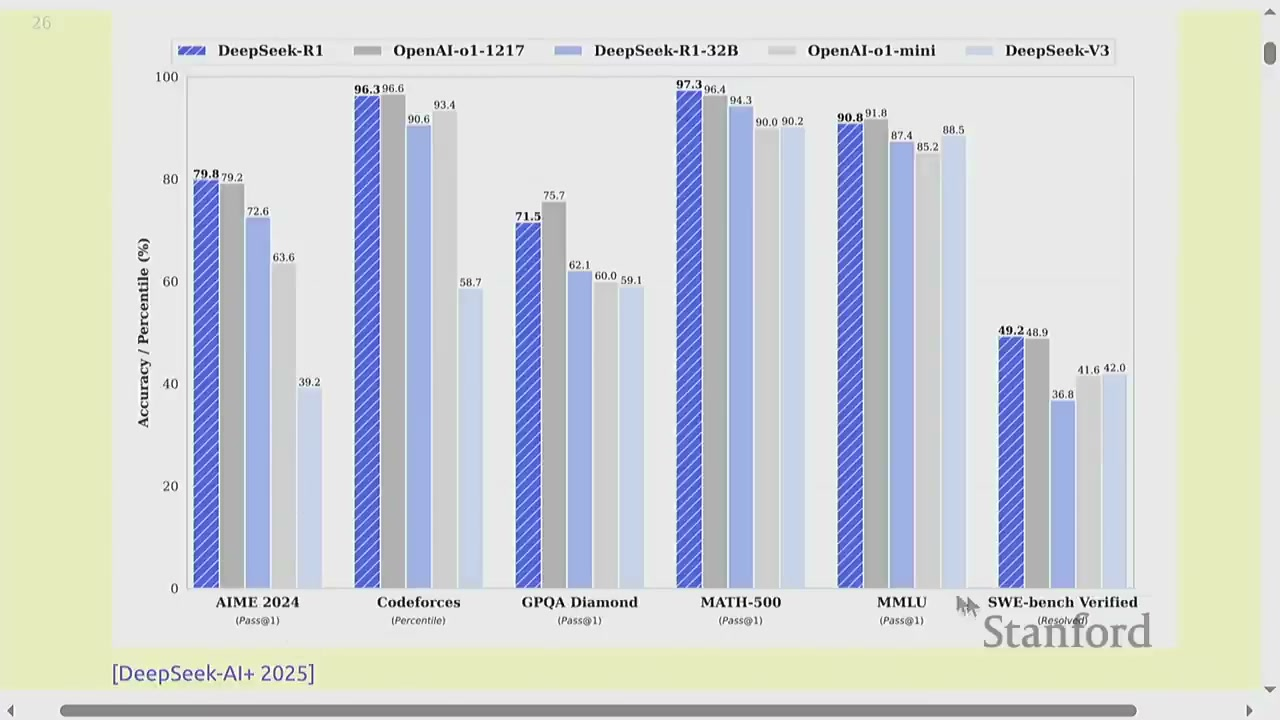
\includegraphics[width=\textwidth]{figures/fig_01_benchmark_scores.jpg}
\caption{论文中的 benchmark 分数：Llama 4 在 MMLU Pro / Math 500 / GPQA 等任务上的成绩\protect\footnotemark}
\end{figure}
\footnotetext{视频画面时间区间：00:00:25--00:00:55。}

但真实情况远比这复杂。随便翻开一篇语言模型论文，你会看到一连串数字——MMLU、HumanEval、Codeforces、DROP、GSM8K、GPQA……大多数模型在大致相同的 benchmark 上评测，但又"不完全一样"。这些数字到底意味着什么？哪一个是"对的"评测方式？这就是本讲要厘清的核心问题。

\subsection{四种看模型好坏的视角}

Percy 在课堂上抛出了一组异质的"好坏信号源"，展示评估生态的碎片化：

\begin{figure}[H]
\centering
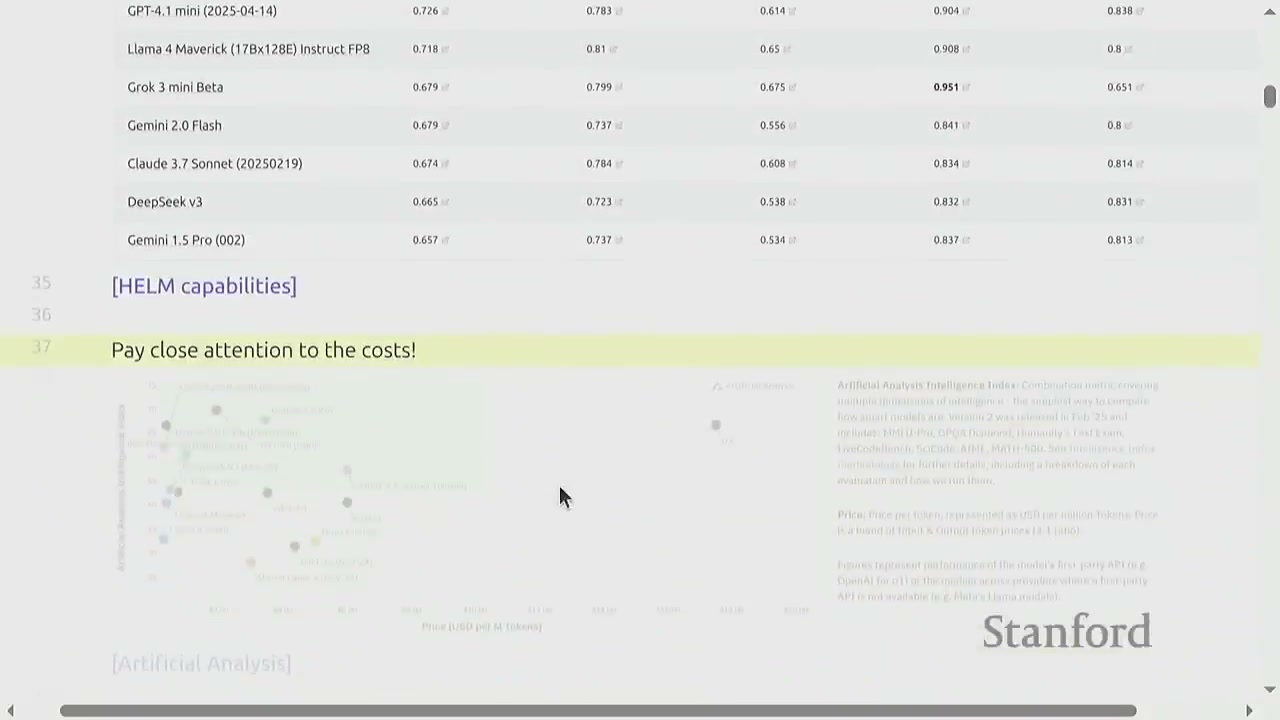
\includegraphics[width=\textwidth]{figures/fig_02_helm.jpg}
\caption{HELM：把多种标准 benchmark 聚合在一起的统一评估平台\protect\footnotemark}
\end{figure}
\footnotetext{视频画面时间区间：00:01:35--00:02:05。}

\begin{figure}[H]
\centering
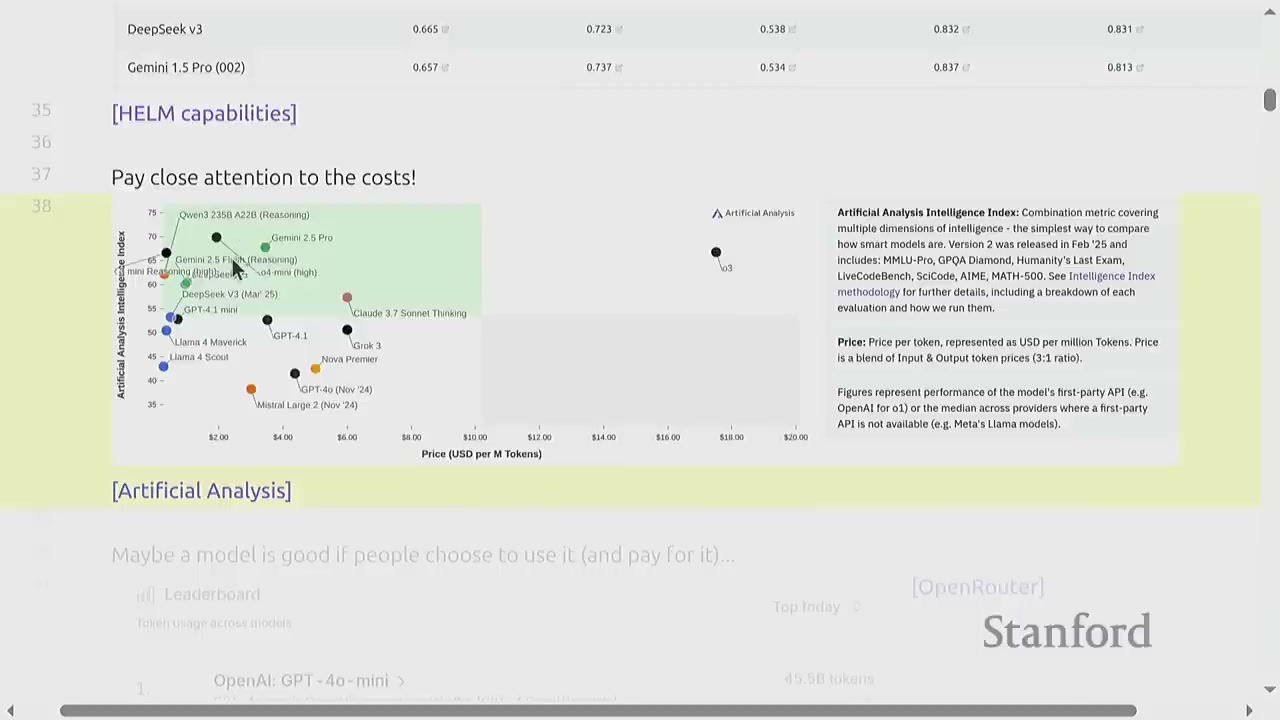
\includegraphics[width=\textwidth]{figures/fig_03_pareto_frontier.jpg}
\caption{Artificial Analysis：横轴价格、纵轴"智能指数"的 Pareto 前沿——不仅看能力，也看成本\protect\footnotemark}
\end{figure}
\footnotetext{视频画面时间区间：00:02:05--00:02:35。}

\begin{figure}[H]
\centering
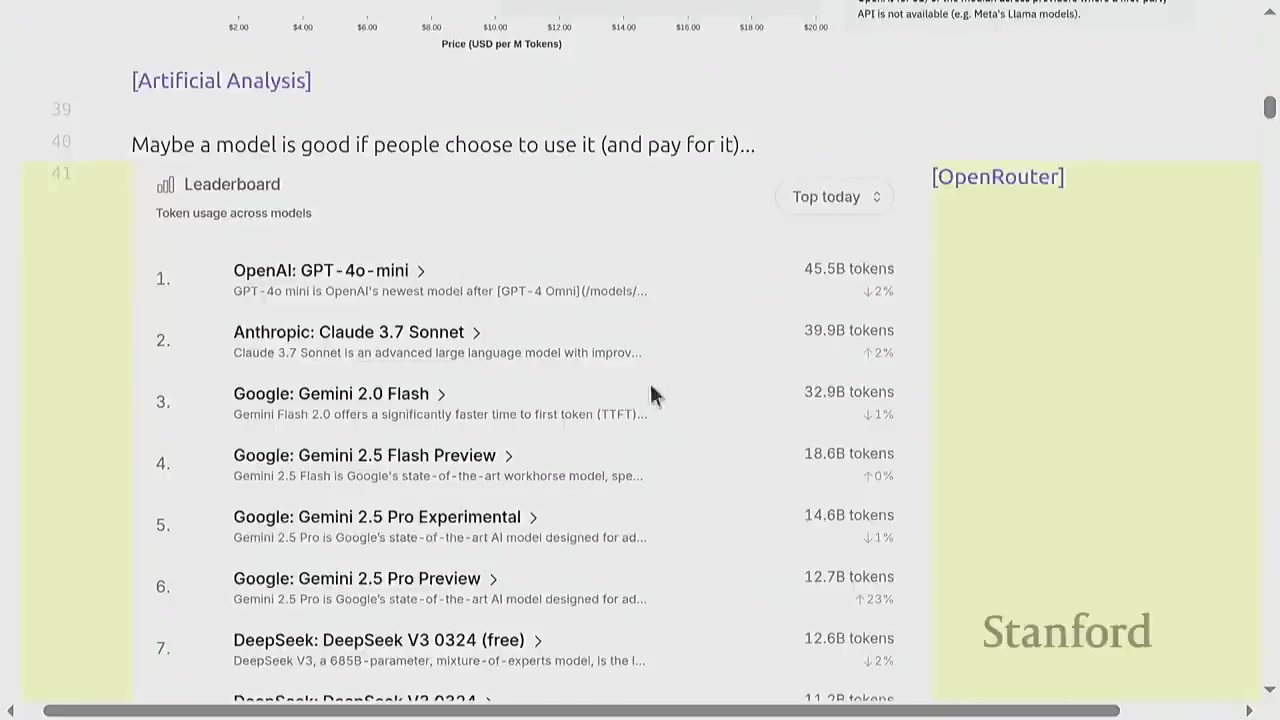
\includegraphics[width=\textwidth]{figures/fig_04_openrouter_traffic.jpg}
\caption{OpenRouter：按人们实际调用各模型的 token 量排序——"好用与否"的隐式投票\protect\footnotemark}
\end{figure}
\footnotetext{视频画面时间区间：00:02:45--00:03:15。}

\begin{enumerate}
\item \textbf{论文里的 benchmark 表}：每个实验室自报家门，挑自己想报的指标。
\item \textbf{聚合平台}（HELM）：尽量把多任务、多维度标准化地摆在一起。
\item \textbf{Pareto 前沿}（Artificial Analysis）：能力与价格权衡，o3 很强但也很贵，别的模型可能"够好且便宜得多"。
\item \textbf{使用流量}（OpenRouter）：模型好不好的最终证据，或许是\textbf{人们是否真的在用}。按 token 流量排序，OpenAI、Anthropic、Google 居前。
\item \textbf{Chatbot Arena}：互联网众包的成对偏好，转成 Elo 排名——后面会专门讨论它的问题。
\item \textbf{"vibes"}：X 上的零散案例（"看这个模型多强"），并非系统评测。
\end{enumerate}

\subsection{评估危机}

\begin{figure}[H]
\centering
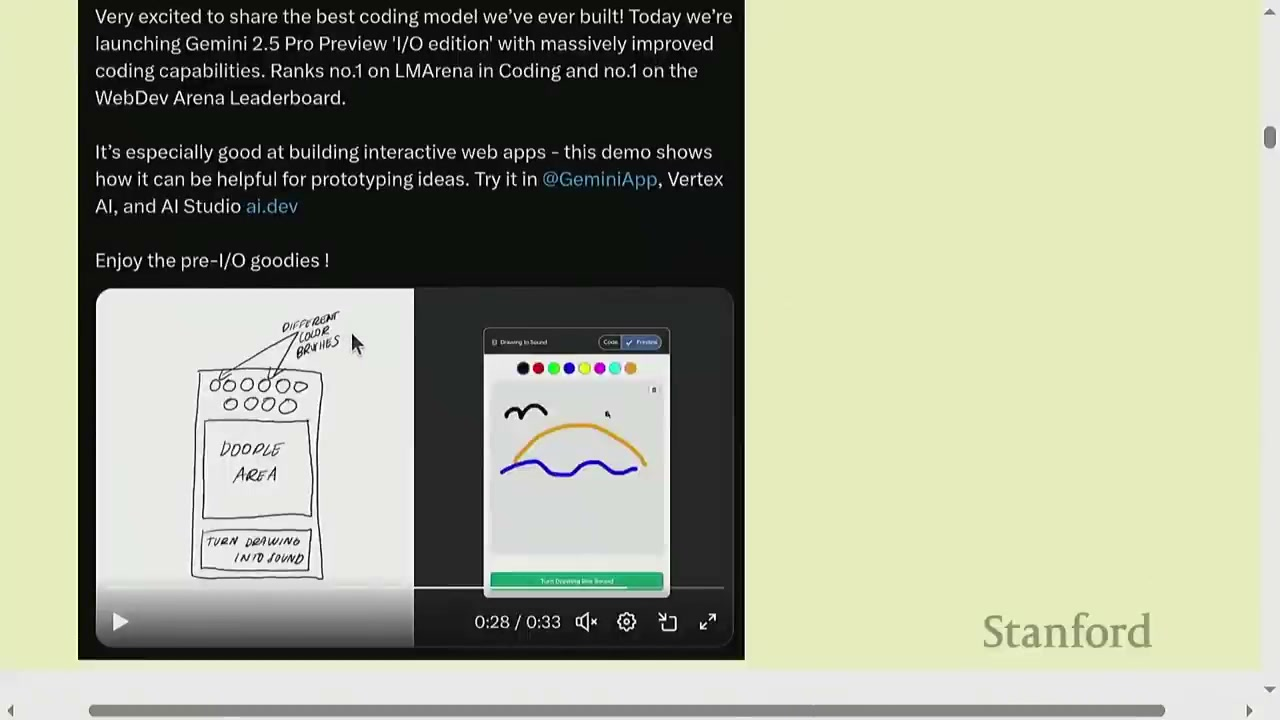
\includegraphics[width=\textwidth]{figures/fig_05_eval_crisis.jpg}
\caption{Karpathy 的判断：我们正处于"评估危机"——benchmark 被饱和或被博弈\protect\footnotemark}
\end{figure}
\footnotetext{视频画面时间区间：00:03:25--00:03:55。}

Percy 引用 Andrej Karpathy 的判断：当下存在\textbf{评估危机（evaluation crisis）}。曾经的金标准如 MMLU，其底层假设已被动摇——要么\textbf{饱和}（所有人都 90\%+，无法区分），要么\textbf{被博弈}（goodhart's law：一旦某个指标被当成目标优化，它就不再是好指标），要么介于二者之间。Chatbot Arena 也问题重重。

\begin{warningbox}{Goodhart 定律的评估版}
当一个评测变成被追踪、被优化的目标，它就立刻失去作为"真理"的资格。模型开发者会盯着 leaderboard 做决策，于是 leaderboard 反过来塑造了模型——这正是评估为何是"未来走向的领先指标"。
\end{warningbox}

Percy 强调本课的一个贯穿性主题：\textbf{一切都 messy}，评估也不例外。

\subsection{评估为什么决定了模型怎么被造}

评估不只是事后的"打分牌"。它深刻地\textbf{反向塑造}模型开发：前沿实验室追踪这些指标随时间的变化，试图让自己的数字上升；于是指标指导了开发决策。评估因而是一个\textbf{领先指标（leading indicator）}，预示着技术往哪走。

\section{评估的概念框架}

\subsection{没有唯一正确的评估}

\begin{figure}[H]
\centering
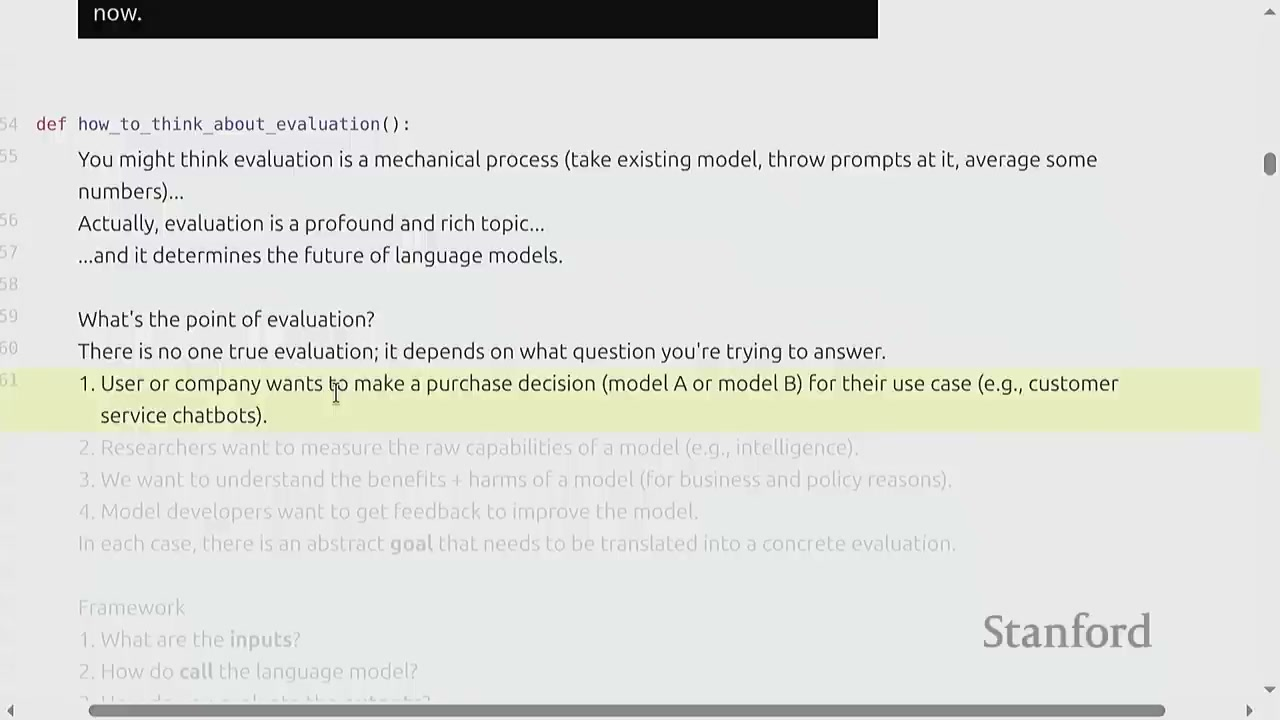
\includegraphics[width=\textwidth]{figures/fig_06_no_one_eval.jpg}
\caption{没有"一个真实评估"：评估取决于你想回答什么问题\protect\footnotemark}
\end{figure}
\footnotetext{视频画面时间区间：00:06:25--00:06:55。}

\begin{importantbox}{核心命题}
\textbf{不存在"那个唯一的评估"。}评估的好坏，取决于它是否回答了你最初想问的问题。"我只是在评估一个模型"——这句话本身没有意义，因为脱离了目标，那个数字什么也不说明。
\end{importantbox}

Percy 列举了四类典型的评估动机，每类背后是不同的"问题"：

\begin{tabular}{p{2.8cm}p{4.5cm}p{6cm}}
\toprule
\textbf{谁在评估} & \textbf{想回答的问题} & \textbf{对应的评估} \\
\midrule
用户/采购方 & Claude、Grok、Gemini、o3 哪个适合我的场景 & 任务特化、成本敏感 \\
研究者 & 模型的原始能力？AI 是否在进步 & 通用、与使用解耦 \\
政策制定者 & 模型的收益与风险现状 & 全面、覆盖能力与安全 \\
模型开发者 & 这个干预有效吗？要不要保留 & 快速、可对比 \\
\bottomrule
\end{tabular}

\subsection{四步评估框架}

\begin{figure}[H]
\centering
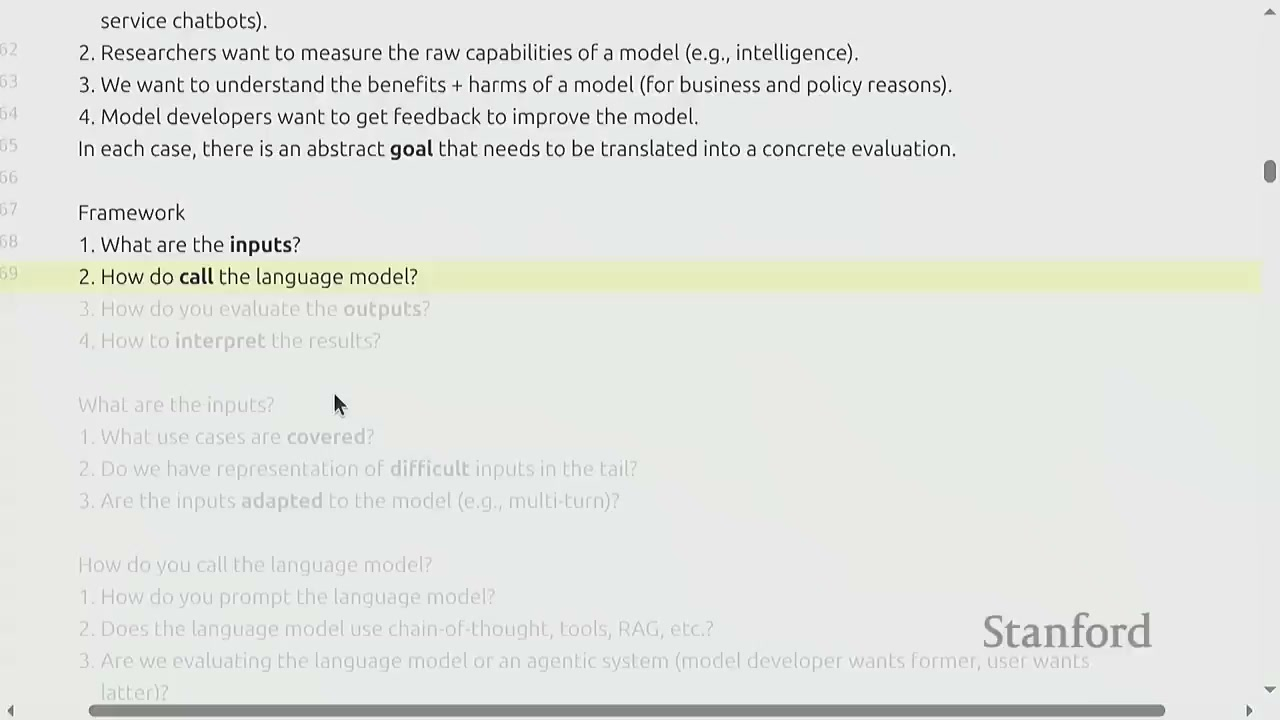
\includegraphics[width=\textwidth]{figures/fig_07_eval_framework.jpg}
\caption{评估的统一框架：输入 $\to$ 调用模型 $\to$ 评估输出 $\to$ 解读结果\protect\footnotemark}
\end{figure}
\footnotetext{视频画面时间区间：00:08:15--00:08:45。}

Percy 给出一个简单的四步框架，每一步都藏着陷阱：

整体可抽象为一条从输入到分数的管线。设输入分布 $Q$、模型 $M_\theta$、调用策略 $\pi$（few-shot/CoT/工具）、评分函数 $s$，则评估就是对该管线的期望：

\[
\text{Score}(M_\theta) = \mathbb{E}_{q \sim Q}\!\left[ s\big( \pi(M_\theta, q),\; q \big) \right]
\]

\begin{itemize}
\item $q$：从输入分布 $Q$ 采样的 prompt
\item $\pi(M_\theta, q)$：在策略 $\pi$ 下、模型 $M_\theta$ 对 $q$ 的调用与生成过程
\item $s(\cdot, q)$：针对题 $q$ 的评分函数（exact match、胜率、测试通过率……）
\item 最终分数是这条管线在输入分布上的期望——每一环的偏差都会污染它
\end{itemize}

\textbf{第一步——输入（inputs）：}prompt 从哪来？覆盖哪些用例？有没有"尾部"困难样本，还是全是 vanilla 简单题？更微妙的是，输入是否要\textbf{适配模型}。多轮对话里输入天然依赖模型；单轮也未必固定。红队（red teaming）里，为模型量身定制 prompt 才能高效触发罕见有害行为——但这又让跨模型比较变得困难。

\begin{knowledgebox}{输入适配的两难}
适配输入 $\to$ 触发尾部事件更高效；但不适配 $\to$ 不同模型才可比。这是评估设计中无处不在的张力。
\end{knowledgebox}

\textbf{第二步——调用模型（calling the LM）：}零样本、少样本、思维链（CoT）？是否允许工具调用（计算器、代码执行、检索增强）？这些决策会引入\textbf{巨大的方差}。语言模型对 prompt 极其敏感，评估必须把这种敏感性纳入考量。

\textbf{第三步——评估输出（assessing outputs）：}参考答案干净吗、无错吗？代码生成用 pass@1 还是 pass@10？成本是否被考虑？leaderboard 常把成本"边际化"掉，于是你看不到第一名可能比第二名贵 10 倍。开放生成（"写一个关于 Stanford 的故事"）没有 ground truth，怎么评？

代码生成中的 pass@$k$ 定义为：从模型采样 $n$ 个候选解，其中至少有一个通过测试的概率：

\[
\text{pass@}k = 1 - \frac{\binom{n-c}{k}}{\binom{n}{k}}
\]

\begin{itemize}
\item $n$：总采样数；$c$：其中正确的个数；$k$：允许选取的个数
\item $\binom{n-c}{k}/\binom{n}{k}$：在 $n$ 中随机取 $k$ 个\textbf{全部取错}的概率
\item pass@1 最严苛（一次就要对），pass@10 宽松得多——选不同的 $k$ 会得到截然不同的"代码能力"结论
\end{itemize}

\textbf{第四步——解读结果（interpreting results）：}拿到 91 分，够用吗？能上线吗？是否真的学到了某种泛化？这要求直面\textbf{训练-测试重叠（train-test overlap）}。还有：你评的到底是模型、是系统、还是方法？研究论文的产出常是一个新\textbf{方法}，模型只是它的载体——没有清晰对照，评估就没意义。

\begin{importantbox}{评估对象的三重性}
\begin{itemize}
\item \textbf{模型（model）}：开发者关心的对象，scaffolding 只是手段。
\item \textbf{系统（system）}：用户关心的对象，可能含多个模型 + 工具，只看端到端效果。
\item \textbf{方法（method）}：研究者关心的对象，需要严格控制才能分离出方法的贡献。
\end{itemize}
混淆这三者，是评估中最常见的概念错误。
\end{importantbox}

\section{Perplexity：最古老的语言模型指标}

\subsection{Perplexity 是什么}

\begin{figure}[H]
\centering
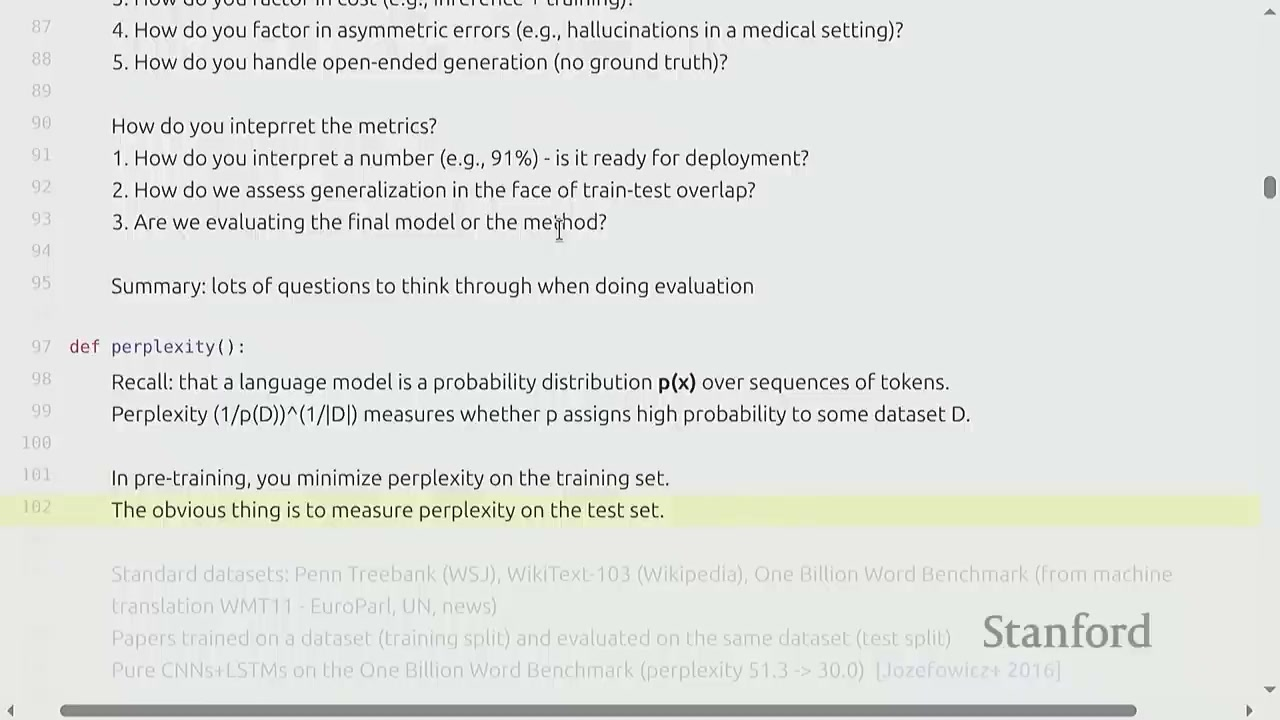
\includegraphics[width=\textwidth]{figures/fig_08_perplexity.jpg}
\caption{Perplexity：语言模型对测试集分配的概率（对数似然的指数）\protect\footnotemark}
\end{figure}
\footnotetext{视频画面时间区间：00:16:45--00:17:15。}

语言模型本质上是一个\textbf{token 序列上的概率分布}。Perplexity 衡量的是：模型对某个数据集（通常是验证集或测试集）分配了多高的概率。形式化地，给定长度为 $L$ 的测试序列 $\mathbf{x} = (x_1, \ldots, x_L)$，模型参数为 $\theta$：

\[
\log p_\theta(\mathbf{x}) = \sum_{t=1}^{L} \log p_\theta(x_t \mid x_{<t})
\]

\begin{itemize}
\item $p_\theta(x_t \mid x_{<t})$：模型在给定前缀 $x_{<t}$ 时预测位置 $t$ 的条件概率
\item $\log p_\theta(\mathbf{x})$：序列的对数似然，越大说明模型越"认可"这串数据
\end{itemize}

定义每个 token 的平均负对数似然，再取指数即为 perplexity：

\[
\mathrm{PPL}(\mathbf{x}) = \exp\left( -\frac{1}{L} \sum_{t=1}^{L} \log p_\theta(x_t \mid x_{<t}) \right)
\]

\begin{itemize}
\item $\mathrm{PPL}$：困惑度，可理解为"模型在每个位置平均在多少个等概率词之间犹豫"
\item $\mathrm{PPL}=1$ 意味完全确定；越大越困惑
\item 它是\textbf{自回归训练目标}的直接延伸，因此预训练就是在最小化训练集的 perplexity
\end{itemize}

\begin{knowledgebox}{为什么用交叉熵的指数？}
负对数似然（NLL）即交叉熵 $\mathcal{L}_{\text{CE}}$。取指数 $\exp(\mathcal{L}_{\text{CE}})$ 后，单位从"每 token 比特"变成"等效候选词数"，更直观——PPL=30 意味着模型像在 30 个等可能词里猜。
\end{knowledgebox}

\subsection{2010 年代的 perplexity 黄金期}

\begin{figure}[H]
\centering
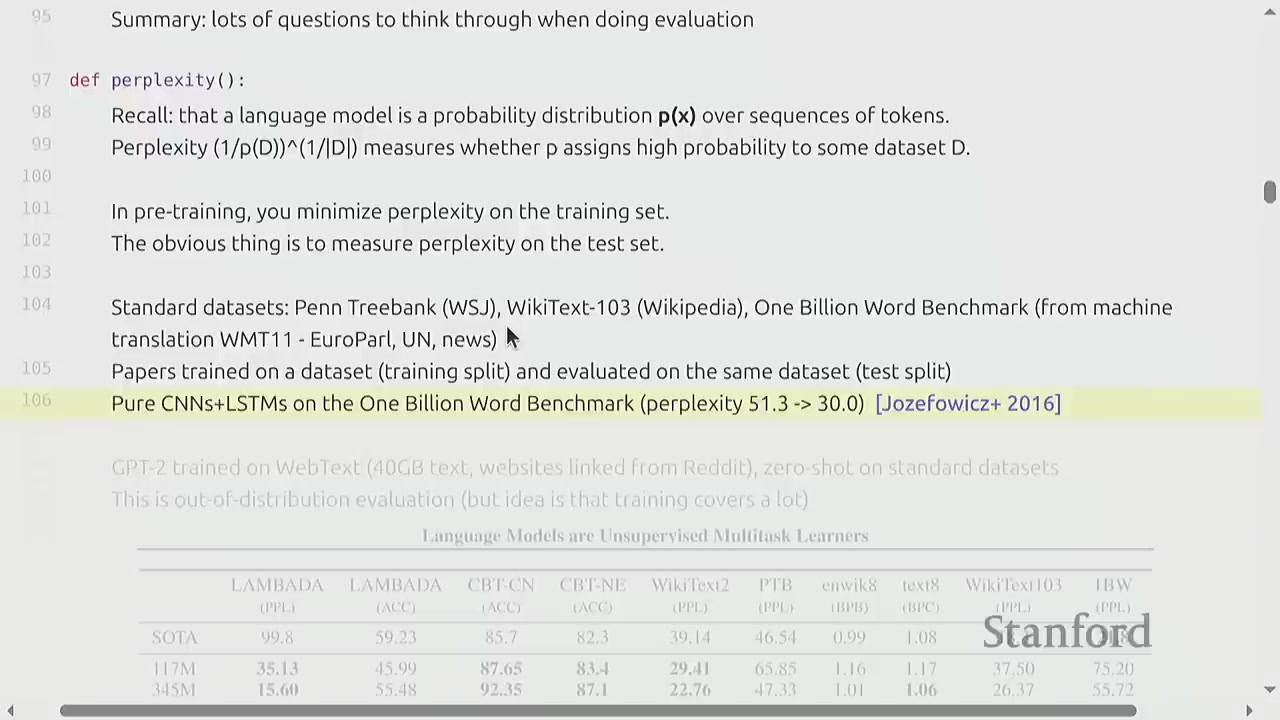
\includegraphics[width=\textwidth]{figures/fig_09_gpt2_zeroshot.jpg}
\caption{GPT-2：在 WebText 上训练后，零样本跨域评测 Penn Treebank / WikiText / 1B Words\protect\footnotemark}
\end{figure}
\footnotetext{视频画面时间区间：00:18:55--00:19:25。}

2010 年代的语言建模研究就建立在一组标准数据集上：\textbf{Penn Treebank}（可追溯到 1990 年代）、\textbf{WikiText}、\textbf{1 Billion Word Benchmark}（源自机器翻译，多为政府公文与新闻）。研究者各取一个数据集，在指定训练 split 上训练，在测试 split 上报 perplexity。

Google 一篇标志性论文表明：只要架构设计得当并放大规模，perplexity 能从 51 大幅降到 30——这是\textbf{断崖式}的进步。Perplexity 作为一个 challenge problem，强力推动了语言建模研究。

\begin{importantbox}{小数据 vs 大数据的两套游戏}
在小数据集上，人们担心\textbf{过拟合}；而在大数据集上，游戏变成"能不能把数据拟合进去"。这是 Percy 强调的范式分野。
\end{importantbox}

\subsection{GPT-1/2 改变了评估范式}

GPT-2 在 40GB 网页文本（Reddit 外链）上训练，然后\textbf{不微调、直接}在 Penn Treebank、WikiText 等标准 benchmark 上评测。这是典型的\textbf{分布外评估}——训练分布是网页，评测分布是学术语料。但训练数据足够广，模型获得了强泛化。

结果是：在 Penn Treebank 等小数据集上，GPT-2 \textbf{零样本就超越}了专门在这些数据上训练的 SOTA；只在 1B Words 上仍略逊。这说明足够广的预训练可以"顺便"赢下狭义任务。Cross-entropy / perplexity 与下游表现的\textbf{弱相关性}也由此埋下伏笔。

\begin{warningbox}{Perplexity 与下游能力的关系并不稳健}
Tatsu 上一讲展示的图表明：perplexity 与下游任务的相关性\textbf{忽高忽低}。只有当跨多个 scale 纵观时，perplexity 才"全局上"对应一切在变好——强模型在大多数事上都强，1B 小模型在大多数事上都弱。但局部、单点上，perplexity 下降未必带来你关心的那个能力的提升。
\end{warningbox}

\subsection{数据污染与去污染}

\begin{figure}[H]
\centering
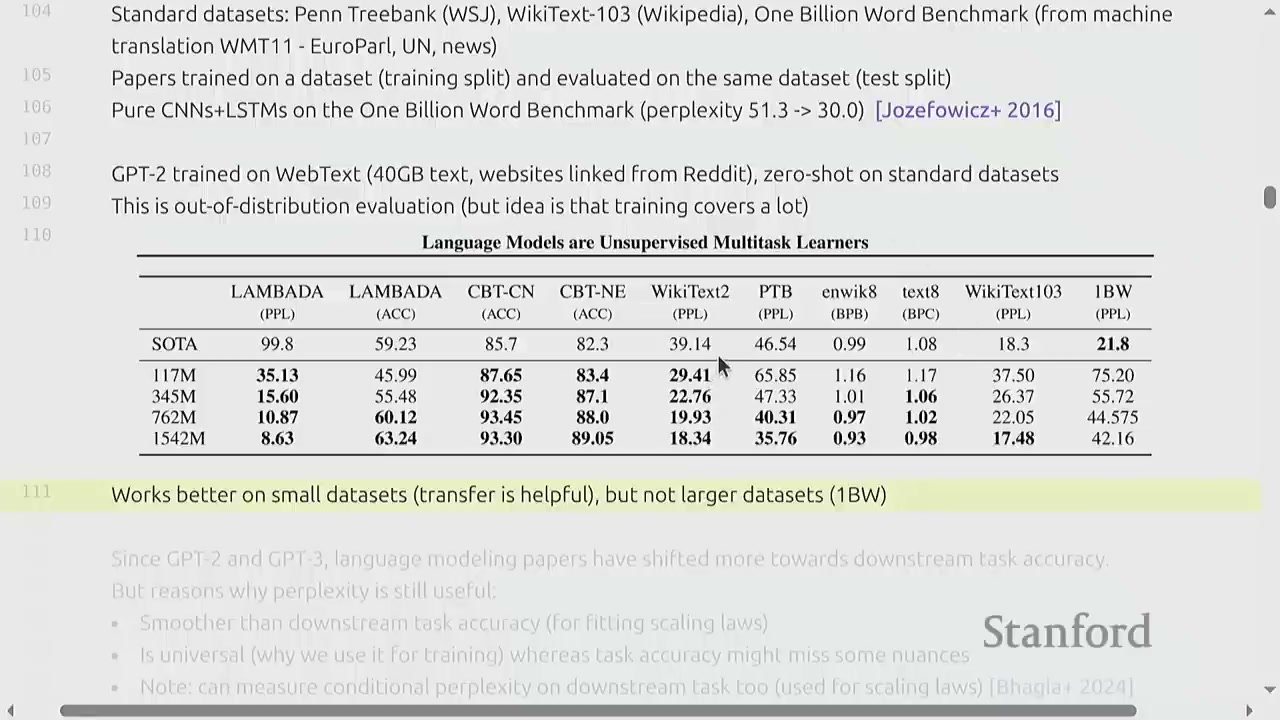
\includegraphics[width=\textwidth]{figures/fig_10_contamination.jpg}
\caption{数据污染（contamination）：测试集泄入训练数据，导致指标虚高\protect\footnotemark}
\end{figure}
\footnotetext{视频画面时间区间：00:21:30--00:23:00。}

\textbf{污染（contamination）}是 perplexity 评估的头号威胁：如果测试集本身就是训练数据的一部分，模型只是"背答案"，perplexity 虚低，但泛化能力为零。标准做法是\textbf{去污染（decontamination）}：把测试集与训练集做比对，移除任何重叠文档。

\begin{importantbox}{保守去污染的原则}
与其纠结"是否真的训过"，不如直接\textbf{保守地}剔除一切可疑重叠。网页文本浩如烟海——即便少训了一些，模型仍能学好。若不剔，perplexity 数字毫无意义。
\end{importantbox}

污染的威胁可以用信息论刻画。设真实数据分布为 $T$、模型分布为 $P$。理想情况下 $P \to T$，交叉熵逼近熵的下界：

\[
H(T, P) = H(T) + D_{\mathrm{KL}}(T \,\|\, P) \geq H(T)
\]

\begin{itemize}
\item $H(T, P)$：交叉熵，即我们最小化的训练目标
\item $H(T)$：真实分布的熵，是 perplexity 的理论下界
\item $D_{\mathrm{KL}}(T \| P)$：KL 散度，衡量模型与真分布的偏离，非负
\end{itemize}

若测试集 $T_{\text{test}}$ 被污染进训练集，模型对它的概率被人为抬高，交叉熵\textbf{低于} $H(T)$——这从数学上就不可能来自真实的泛化，只能是记忆。于是污染让指标违反信息论下界，是可探测的异常。

\subsection{Perplexity 的局限：被回避的难题}

\begin{figure}[H]
\centering
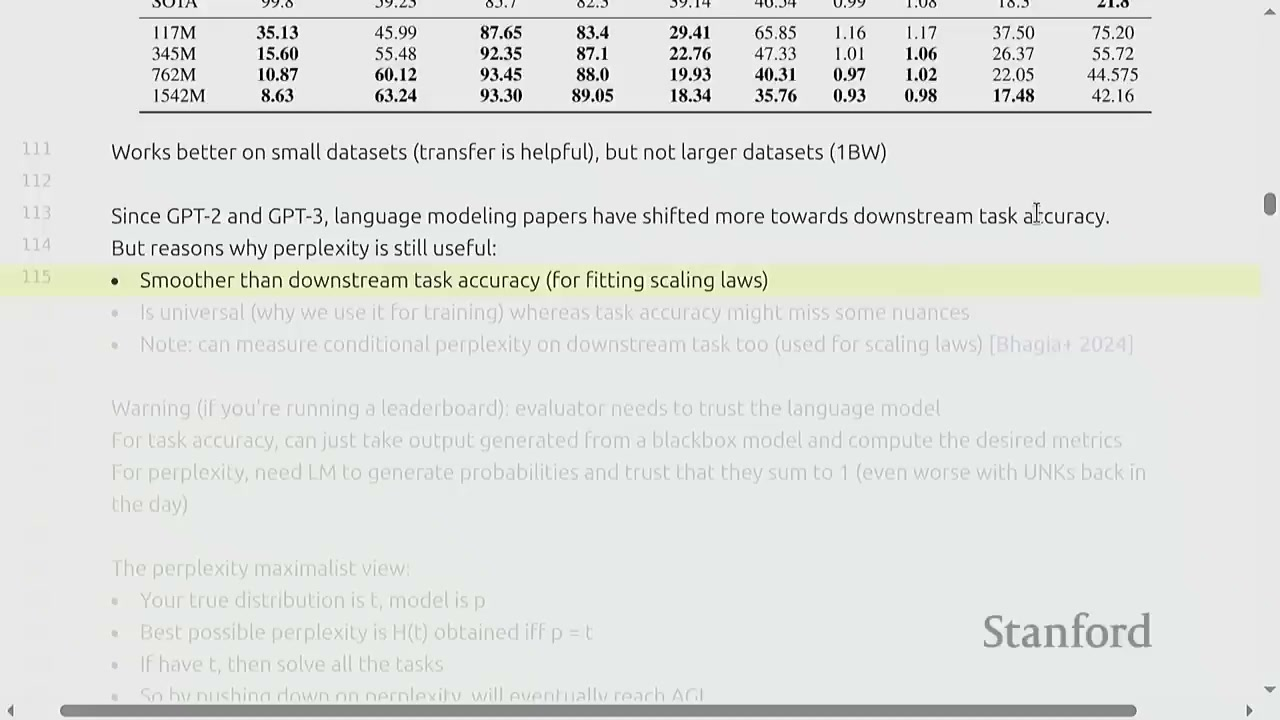
\includegraphics[width=\textwidth]{figures/fig_11_scaling_ppl.jpg}
\caption{Scaling laws 与 perplexity：长程、多尺度上 perplexity 才与能力全局对应\protect\footnotemark}
\end{figure}
\footnotetext{视频画面时间区间：00:24:05--00:24:35。}

Percy 介绍了一类"perplexity 极简主义者（perplexity maximalist）"的立场：与其精心设计下游任务，不如只优化 $D_{\mathrm{KL}}(T \| P)$——即最大化似然。理由是它信息量最大。设 $P$ 为模型分布、$T$ 为真实分布，最大似然等价于最小化交叉熵：

\[
\min_\theta \; H(T, P_\theta) = \min_\theta \; \mathbb{E}_{\mathbf{x} \sim T}\left[ -\log P_\theta(\mathbf{x}) \right]
\]

\begin{itemize}
\item $T$：真实数据分布
\item $P_\theta$：参数 $\theta$ 下的模型分布
\item $H(T, P_\theta)$：交叉熵，最大似然训练的直接目标
\end{itemize}

但反方指出：这可能\textbf{不是最有效}的路径。把概率质量压在不该出现的地方（噪声、低质 token）纯属浪费算力。更糟的是，perplexity 对很多真正重要的能力\textbf{不敏感}——比如指令遵循、安全性、长程推理。

事实上，perplexity 与下游能力 $C$ 之间只存在\textbf{弱、带噪声}的相关，可用一个带噪声的回归刻画：

\[
C \approx \alpha \cdot \big(-\log \mathrm{PPL}\big) + \varepsilon, \quad \mathrm{Var}[\varepsilon] \text{ 较大}
\]

\begin{itemize}
\item $C$：某项下游能力（如 MMLU 准确率）
\item $-\log \mathrm{PPL}$：perplexity 的对数（越高模型越强）
\item $\alpha$：整体正相关斜率，仅在\textbf{跨多个 scale 纵观}时才稳定为正
\item $\varepsilon$：残差噪声，单点上方差大——这就是"perplexity 下降未必带来该能力提升"的数学表达
\end{itemize}

\begin{warningbox}{Perplexity 的三大盲区}
\begin{enumerate}
\item \textbf{对指令/对齐不敏感}：续写得好不等于会回答问题。
\item \textbf{tokenization 耦合}：不同 tokenizer 之间的 perplexity \textbf{不可直接比较}——分词越细，PPL 越低，但这不代表模型更强。
\item \textbf{归一化口径不一}：按 token 平均还是按字符平均，结论可能相反。
\end{enumerate}
\end{warningbox}

为了绕开这些，人们发明了"长得像 perplexity 但不是"的指标——\textbf{cloze（完形）任务}：挖掉句中某个词，看模型能否用条件概率复原它。这把"续写"改造成"填空"，更贴近能力评测。

cloze 准确率只看模型在关键空白处是否把最高概率分配给正确答案：

\[
a_{\text{cloze}} = \mathbb{1}\!\left[ \arg\max_{w \in V} P_\theta(w \mid \text{context}) = w^* \right]
\]

\begin{itemize}
\item $V$：词表；$w^*$：被挖掉的真实词
\item $\arg\max_{w} P_\theta(w \mid \text{context})$：模型在给定上下文下最可能的填词
\item 与 perplexity 不同，这里只关心\textbf{排名第一是否正确}，而非整段概率——更贴近"会不会"而非"续得顺不顺"
\end{itemize}

\[
P_\theta(\text{blank} \mid \text{context}) \quad \text{vs.} \quad P_\theta(\text{full sequence})
\]

\begin{itemize}
\item 左式：cloze 形式，只评估关键位置的条件概率，更聚焦
\item 右式：全序列 perplexity，对所有位置一视同仁
\item cloze 把"评估什么"从"整段续写"聚焦到"特定决策点"，更接近下游能力
\end{itemize}

\section{知识型 Benchmark：MMLU 家族}

\subsection{MMLU 是什么}

\begin{figure}[H]
\centering
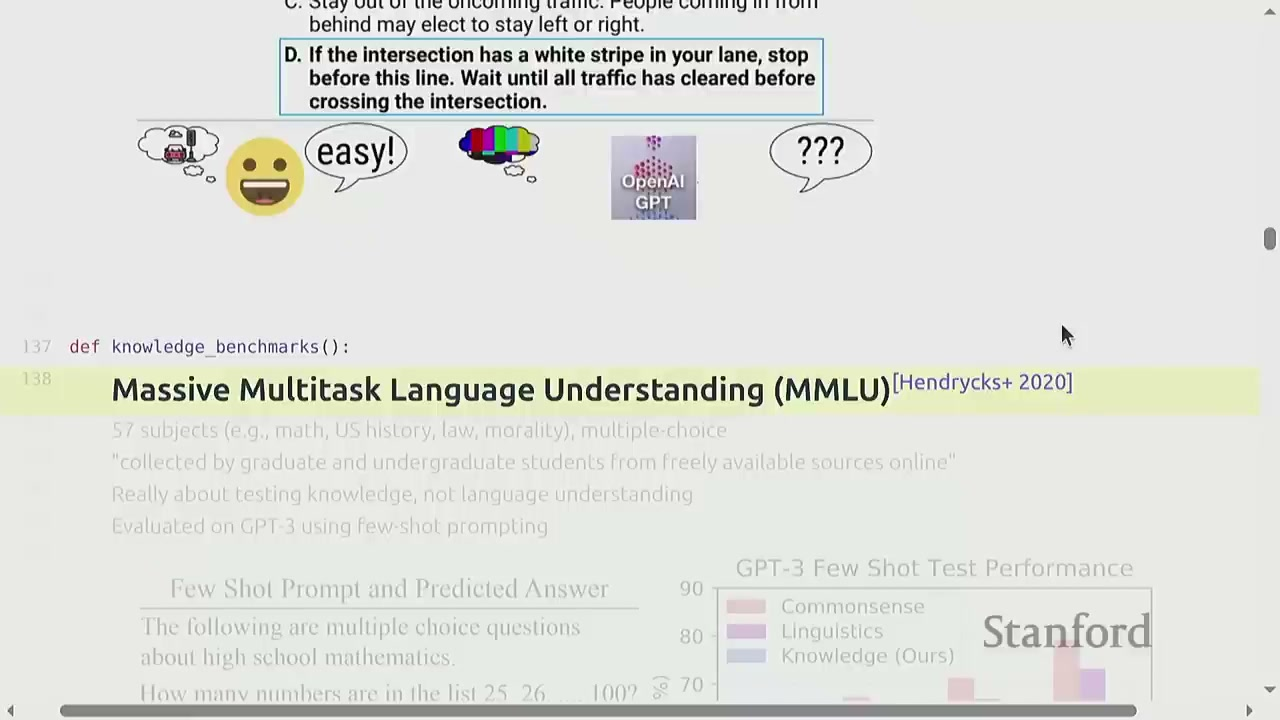
\includegraphics[width=\textwidth]{figures/fig_12_mmlu_intro.jpg}
\caption{MMLU：57 个学科、近 1.6 万道多项选择题的知识 benchmark\protect\footnotemark}
\end{figure}
\footnotetext{视频画面时间区间：00:32:45--00:33:15。}

\textbf{MMLU（Massive Multitask Language Understanding）}是最有影响力的知识型 benchmark：57 个学科（从初等数学到专业医学、法律）、每题 4 选 1。它把"模型懂多少世界知识"压缩成一个准确率数字。

评测时的标准做法是\textbf{少样本提示}（few-shot）：先给模型几道带答案的例题"教它格式"，再让它答新题。

\begin{figure}[H]
\centering
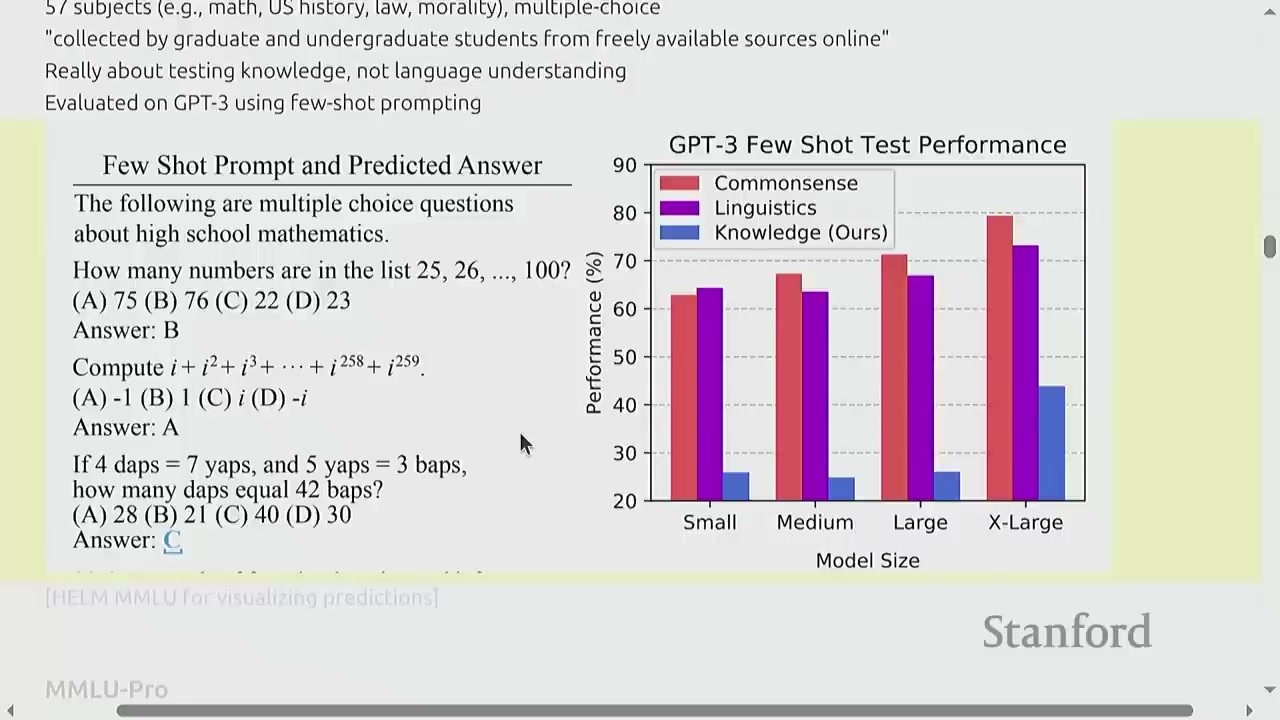
\includegraphics[width=\textwidth]{figures/fig_13_fewshot_prompt.jpg}
\caption{Few-shot prompt 模板：用例题示范输出格式，再让模型作答\protect\footnotemark}
\end{figure}
\footnotetext{视频画面时间区间：00:34:25--00:34:55。}

\subsection{Few-shot 的方差陷阱}

\begin{figure}[H]
\centering
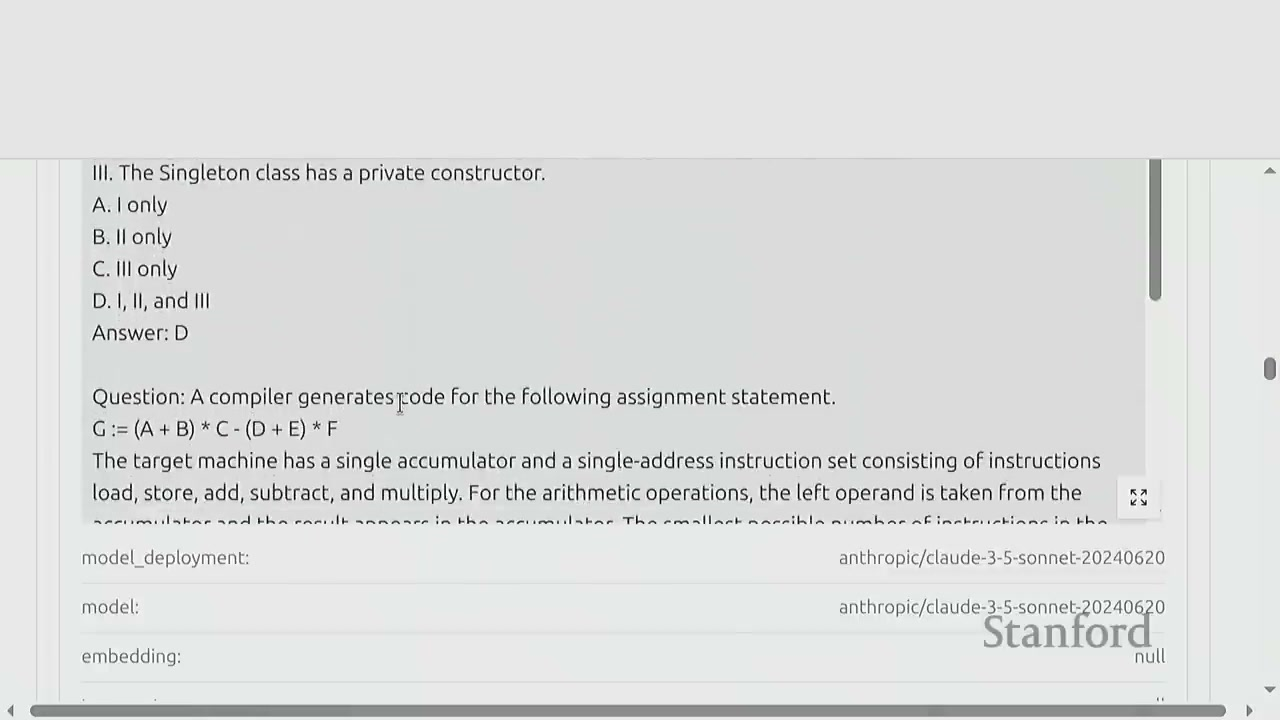
\includegraphics[width=\textwidth]{figures/fig_14_fewshot_variance.jpg}
\caption{Few-shot 示例的\emph{选择}与\emph{顺序}会带来巨大的指标方差\protect\footnotemark}
\end{figure}
\footnotetext{视频画面时间区间：00:37:25--00:37:55。}

Percy 强调一个常被忽视的事实：\textbf{选哪几道例题、按什么顺序放，都会显著改变 MMLU 分数}。同一个模型，换一组 few-shot 例子，分数可能波动好几个点。

\begin{warningbox}{被低估的方差源}
few-shot 例子的\textbf{内容}、\textbf{顺序}、\textbf{数量}都是超参。论文里报一个漂亮数字，往往是最优 few-shot 配置下的"上限"。换配置重跑，分数就变。这让跨论文的 MMLU 比较变得很脆弱。
\end{warningbox}

形式化地，设模型在 prompt 模板 $s$（含特定 few-shot 配置）下的准确率为 $a(s)$，跨配置的标准差反映这一方差源：

\[
\mathrm{Var}_s[a(s)] = \mathbb{E}_s\!\left[ \big(a(s) - \bar{a}\big)^2 \right], \quad \bar{a} = \mathbb{E}_s[a(s)]
\]

\begin{itemize}
\item $s$：某种 few-shot 配置（例子的选择与顺序）
\item $a(s)$：该配置下模型在 benchmark 上的准确率
\item $\mathrm{Var}_s[a(s)]$：跨配置方差，越大说明分数越依赖具体配置，越不可靠
\end{itemize}

不过 Percy 也补充：对现代指令模型而言，few-shot 主要是在\textbf{指定任务格式}——模型已经知道怎么答题，例子只是"说明书"。指令越强，对例子的依赖越弱。

\subsection{MMLU 的时代错位}

\begin{figure}[H]
\centering
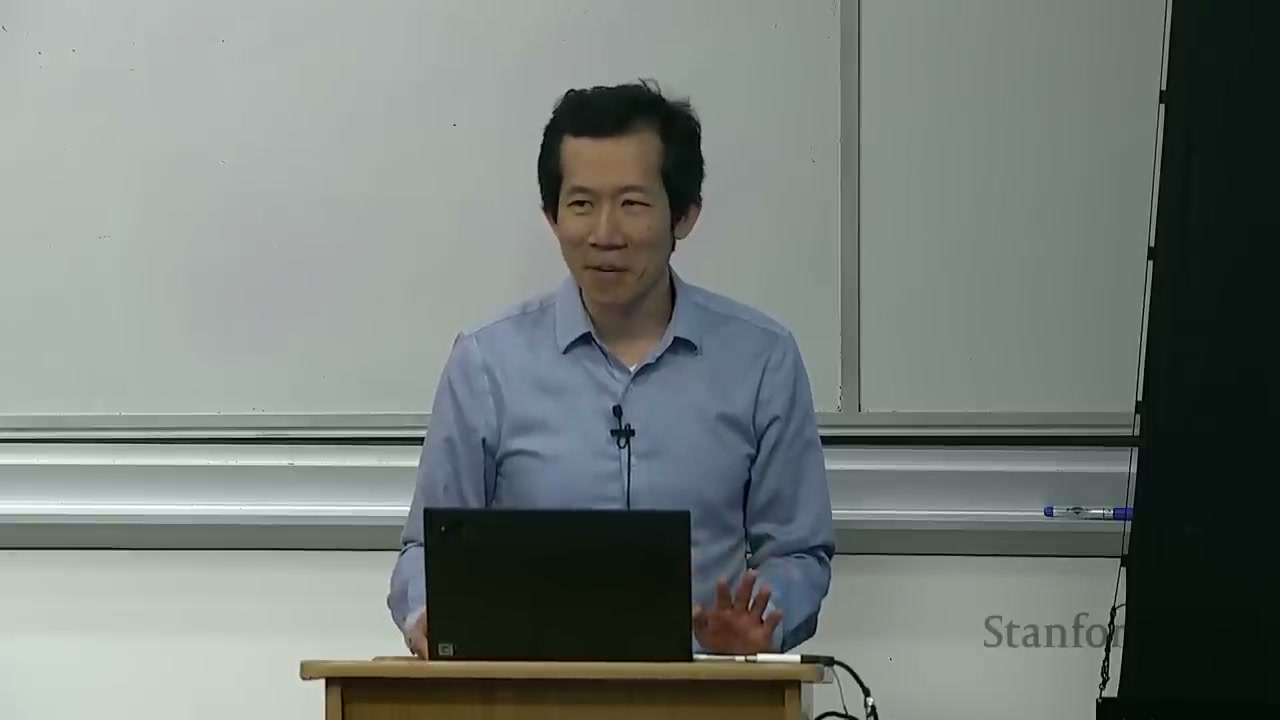
\includegraphics[width=\textwidth]{figures/fig_15_mmlu_2020.jpg}
\caption{MMLU 始于 2020 年——那时还没有指令模型，它是为 base model 设计的\protect\footnotemark}
\end{figure}
\footnotetext{视频画面时间区间：00:40:15--00:40:45。}

\begin{importantbox}{MMLU 的设计前提已过时}
MMLU 创立于 2020 年，彼时\textbf{没有指令模型}。它的 few-shot 形式是为评测 base model 设计的。今天用指令模型去刷它，某种意义上是"用错时代的工具考错时代的卷"。
\end{importantbox}

这就引出了 MMLU 的饱和问题：随着模型变强，MMLU 分数集体逼近 90\%+，区分度消失。社区的反应是\textbf{造更难的版本}。

\subsection{MMLU-Pro 与更难的变体}

\begin{figure}[H]
\centering
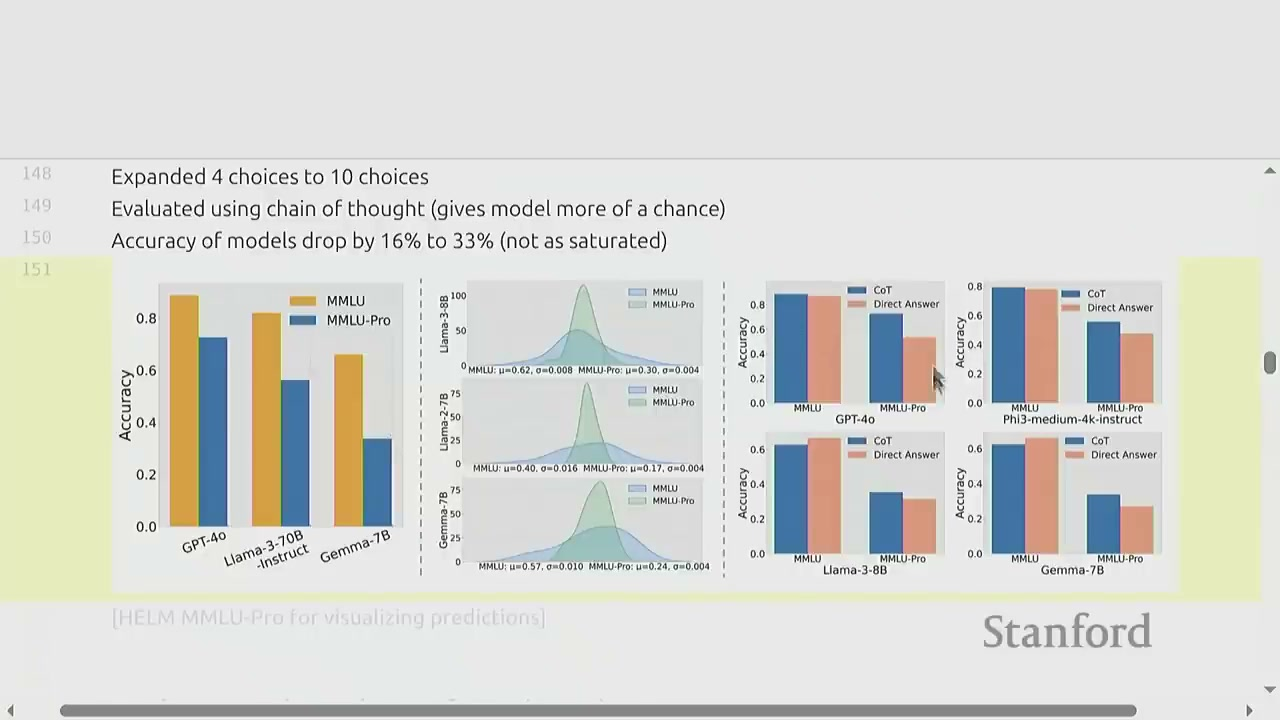
\includegraphics[width=\textwidth]{figures/fig_16_mmlu_pro.jpg}
\caption{MMLU-Pro：剔除噪声题、扩到 10 选项，把饱和区重新拉开\protect\footnotemark}
\end{figure}
\footnotetext{视频画面时间区间：00:41:45--00:42:15。}

\textbf{MMLU-Pro} 的做法：删除原 MMLU 中嘈杂、平庸的简单题，把选项从 4 个扩到 10 个（大幅降低蒙对概率），重新拉开区分度。

随机蒙对的期望准确率随选项数 $K$ 下降，使饱和天花板变高：

\[
a_{\text{random}} = \frac{1}{K}, \quad a_{\text{ceiling}} \approx 1 - \frac{1}{K}
\]

\begin{itemize}
\item $K$：每题的选项数（MMLU 为 4，MMLU-Pro 为 10）
\item $a_{\text{random}}$：纯随机蒙对的期望准确率——$K=4$ 时 0.25，$K=10$ 时 0.10
\item $a_{\text{ceiling}}$：可区分的有效天花板——选项越多，越能拉开"真懂"与"蒙对"的差距
\end{itemize}

\begin{figure}[H]
\centering
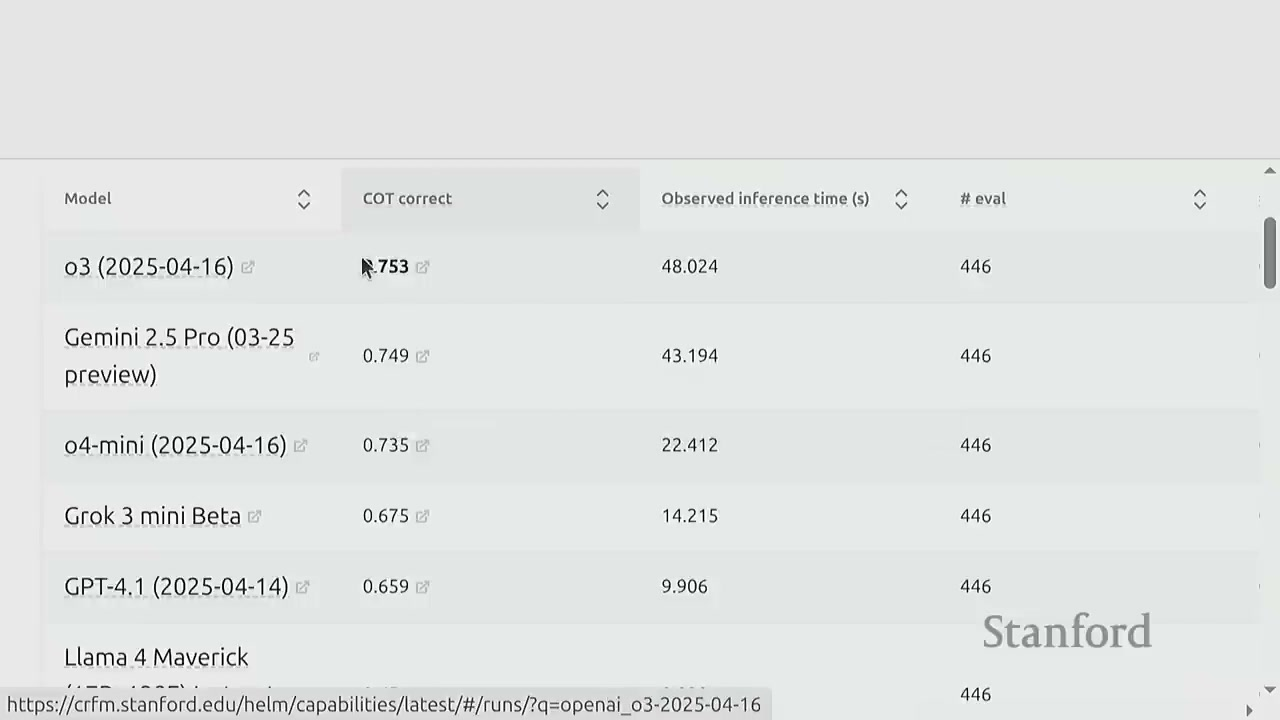
\includegraphics[width=\textwidth]{figures/fig_17_gpqa.jpg}
\caption{GPQA Diamond：研究生水平的专家级问题，人类博士也只能答对约 65\%\protect\footnotemark}
\end{figure}
\footnotetext{视频画面时间区间：00:44:25--00:44:55。}

\textbf{GPQA（Google-Proof Q\&A）}更进一步：由领域专家出题，难度达到\textbf{研究生水平}，即便给人类专家 Google 检索也答不全对。它专门为对抗"模型靠检索/记忆蒙混"而设计。Percy 提到，最近一年 o3 已把 GPQA 推到 75\%。

\begin{figure}[H]
\centering
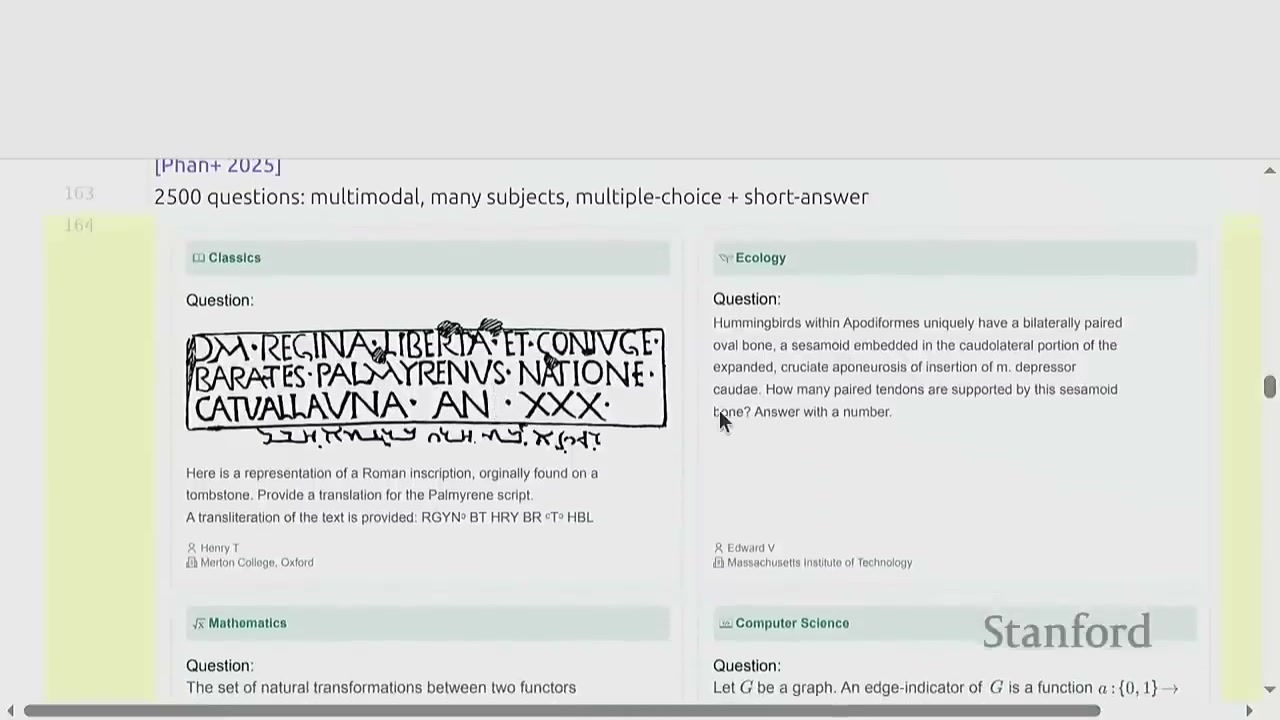
\includegraphics[width=\textwidth]{figures/fig_18_hle.jpg}
\caption{Humanity's Last Exam：向全球征集的极致难题集\protect\footnotemark}
\end{figure}
\footnotetext{视频画面时间区间：00:49:15--00:49:45。}

\textbf{Humanity's Last Exam（HLE）}则是另一个极端：向全球开放征集"最难"的题，每题都需专家多轮审校。Percy 直言这类数据集的创建\textbf{极其耗时}，且设计哲学几乎与他从第一性原理出发的设计相反——开放征集天然引入偏见。它们"确实很难"，但\textbf{不代表任何现实分布}。

\begin{knowledgebox}{难题集的两难}
难题集解决了"饱和"问题，却引入了\textbf{代表性}问题：满纸精英级偏题，与普通人、普通场景脱节。"难"不等于"有用"。这正是评估永恒的张力——区分度 vs 真实性。
\end{knowledgebox}

\section{开放生成与人类偏好}

\subsection{核心难题：开放生成怎么评}

\begin{importantbox}{开放生成的评估困境}
"写一个关于 Stanford 的好故事"——没有标准答案。exact match 失效，F1 失效。怎么把"好不好"变成一个数字？这是整个评估领域最难、也最实际的问题。
\end{importantbox}

Percy 介绍了几条主要路线。

\subsection{Chatbot Arena：众包偏好与 Elo}

\begin{figure}[H]
\centering
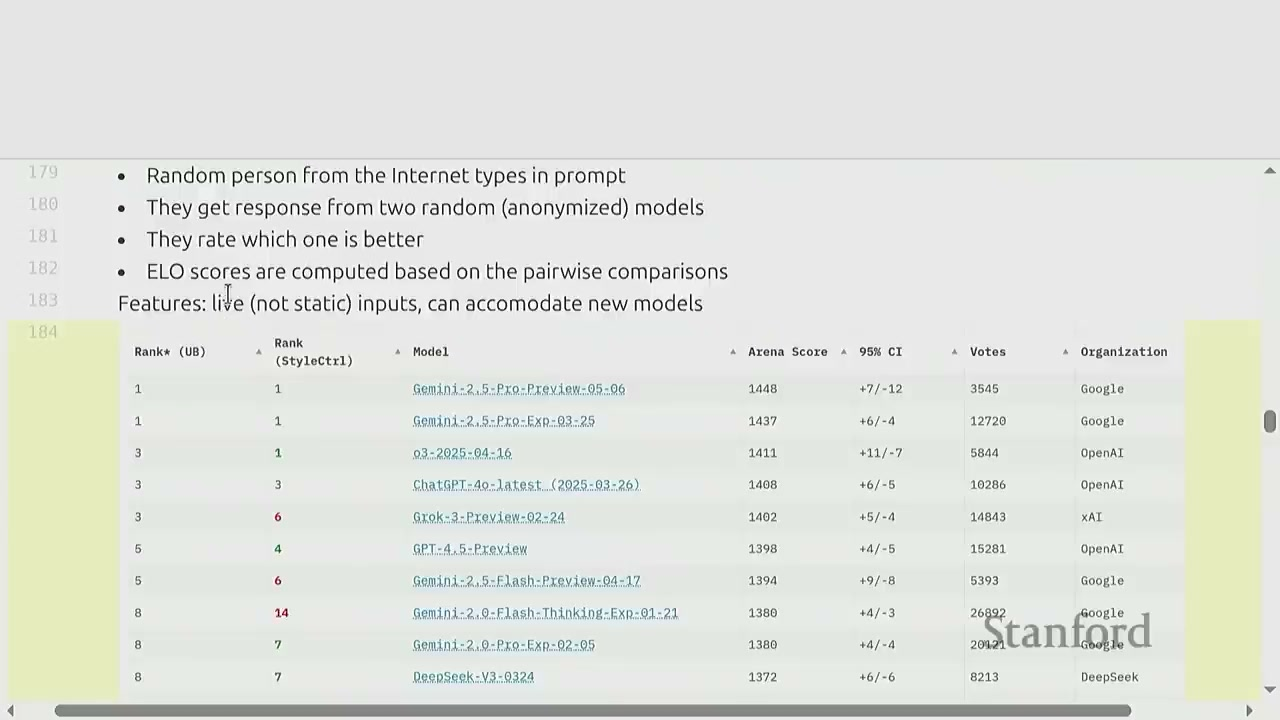
\includegraphics[width=\textwidth]{figures/fig_19_chatbot_arena.jpg}
\caption{Chatbot Arena：用户与两个匿名模型对话，表达成对偏好，汇总成 Elo 排名\protect\footnotemark}
\end{figure}
\footnotetext{视频画面时间区间：00:53:55--00:54:25。}

\textbf{Chatbot Arena}（LMSYS）是最流行的人类评估：用户同时与两个匿名模型对话，选出更喜欢的那个，这些成对偏好用\textbf{Elo 评分系统}（国际象棋同款）聚合成全局排名。它的优点是\textbf{持续刷新}（总有新数据和新模型），能容纳开放生成。

Elo 的核心更新规则：设模型 A 当前评分 $R_A$、模型 B 为 $R_B$，A 的期望胜率（被偏好概率）为

\[
E_A = \frac{1}{1 + 10^{(R_B - R_A)/400}}
\]

\begin{itemize}
\item $E_A$：模型 A 的期望得分（介于 0、1）
\item $R_A, R_B$：双方当前 Elo 评分
\item $400$：标尺常数，表示评分差 400 时强方期望胜率约 0.91
\end{itemize}

每场对局后按实际结果 $S_A \in \{0, 0.5, 1\}$ 更新：

\[
R_A' = R_A + K\,(S_A - E_A)
\]

\begin{itemize}
\item $S_A$：A 的实际结果（胜 1、平 0.5、负 0）
\item $K$：更新步长，越大则单场影响越大
\item 评分差最终反映"被偏好的稳定程度"
\end{itemize}

这一期望胜率公式源自\textbf{Bradley-Terry 模型}：把"被偏好"建模成评分差的 logistic。若用强度参数 $\lambda_A$ 替代评分（$R_A = 400\log_{10}\lambda_A$），A 胜 B 的概率即正比于强度比：

\[
\Pr(A \succ B) = \frac{\lambda_A}{\lambda_A + \lambda_B}
\]

\begin{itemize}
\item $\lambda_A, \lambda_B$：A、B 的潜在"实力"强度参数
\item $\Pr(A \succ B)$：在成对比较中 A 被偏好的概率
\item 这个模型是 Elo、Chatbot Arena 排名、以及很多成对偏好评估的共同数学基础
\end{itemize}

\begin{warningbox}{Chatbot Arena 的问题}
\begin{itemize}
\item \textbf{长度偏好}：人类倾向更喜欢\textbf{更长}的回答，于是模型学会注水。
\item \textbf{风格偏好}：格式、语气、排版（emoji、列表）干扰判断。
\item \textbf{众包质量}：用户的偏好未必专业，可能被表面质量蒙蔽。
\item \textbf{可被 PR 化}：厂商把高排名当营销素材，于是 Goodhart 效应再次降临。
\end{itemize}
\end{warningbox}

\subsection{IFEval：指令遵循的可验证测试}

\begin{figure}[H]
\centering
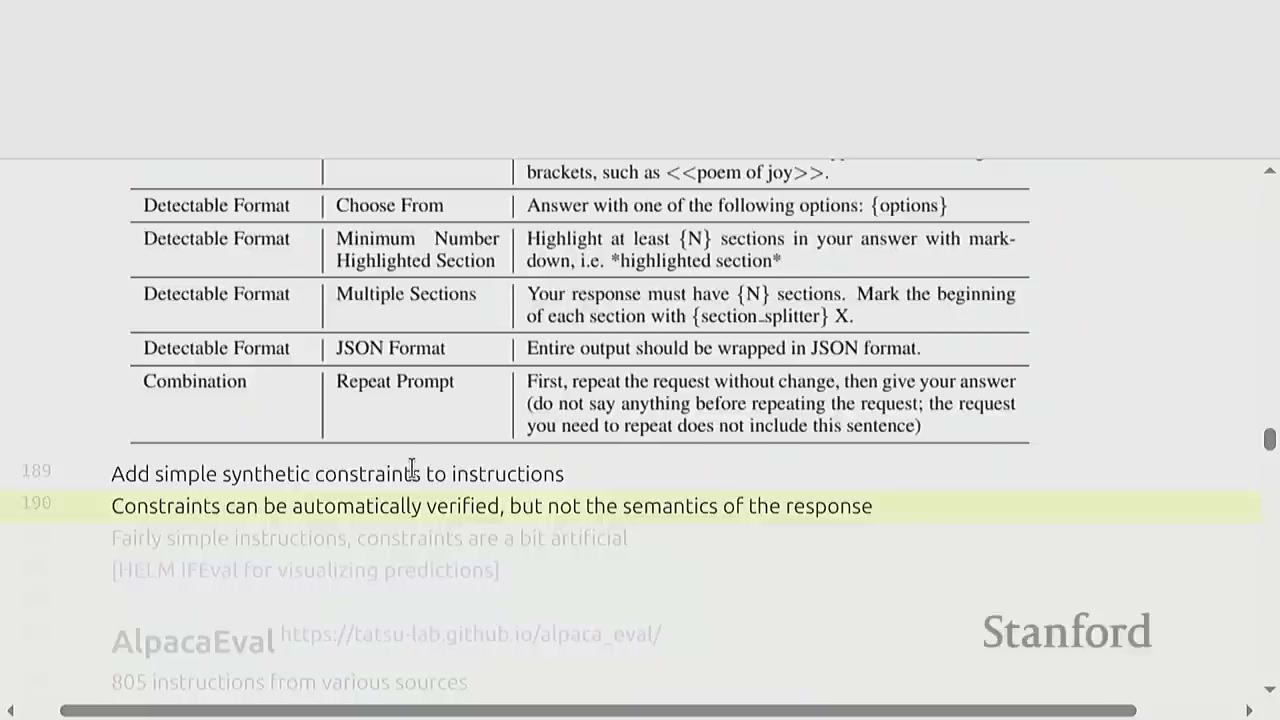
\includegraphics[width=\textwidth]{figures/fig_20_ifeval.jpg}
\caption{IFEval：用可程序化验证的指令（"写一段恰好 10 个词的故事"）测指令遵循\protect\footnotemark}
\end{figure}
\footnotetext{视频画面时间区间：00:56:55--00:57:25。}

\textbf{IFEval} 走另一条路：构造\textbf{可被代码自动验证}的指令，比如"写一段恰好 10 个词的故事"——评分就是\textbf{词数是否等于 10}。它窄而精确，不评"故事好不好"，只评"约束是否被满足"。这类功能测试（functional test）回避了主观判断，可复现、可自动化。

\subsection{AlpacaEval / WildBench：LLM-as-judge}

\begin{figure}[H]
\centering
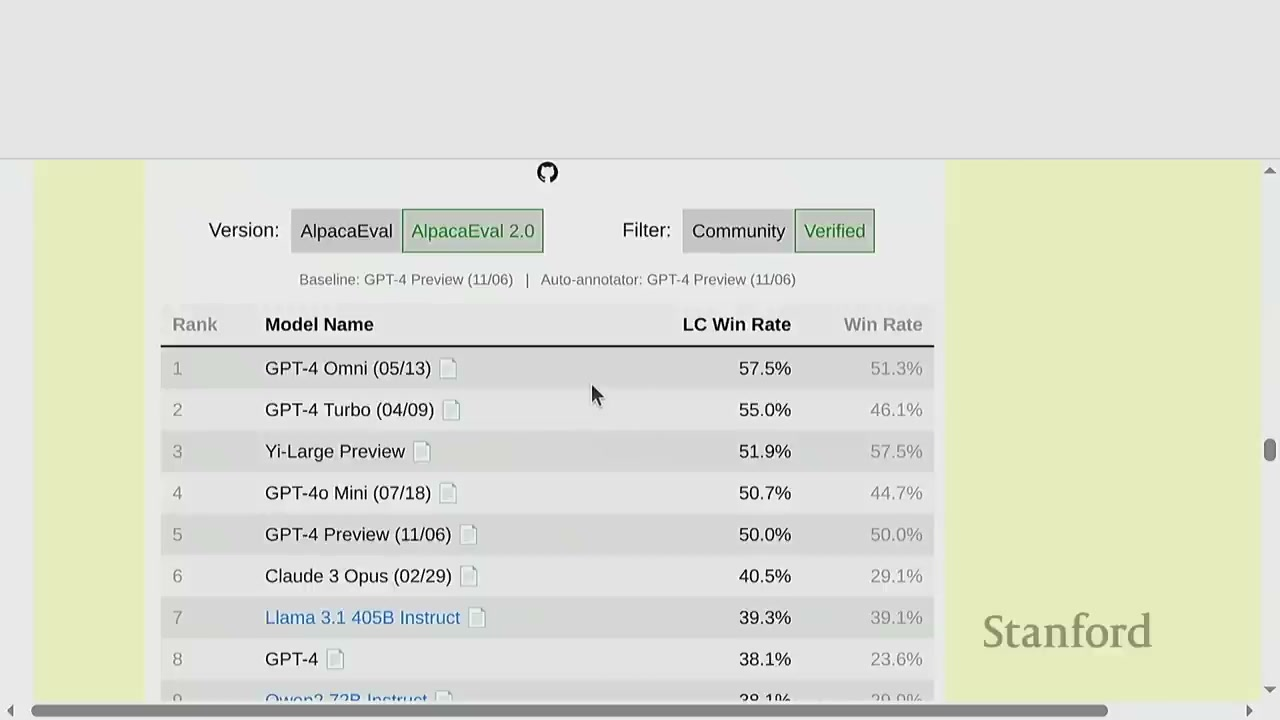
\includegraphics[width=\textwidth]{figures/fig_21_alpacaeval.jpg}
\caption{AlpacaEval：用一个 LLM（如 GPT-4）当裁判，计算被评模型相对基线的胜率\protect\footnotemark}
\end{figure}
\footnotetext{视频画面时间区间：00:58:45--00:59:15。}

\textbf{AlpacaEval} 直接拥抱"LLM 当裁判"：让一个强模型（如 GPT-4）评判被测模型的回答是否优于某个固定基线，输出一个\textbf{胜率（win rate）}。这把开放生成评估自动化了。

胜率定义为被测模型 $M$ 在裁判 $J$ 眼中胜过基线 $B$ 的比例：

\[
\mathrm{WR}(M) = \Pr_{q \sim Q}\!\left[ J(q, M) \succ J(q, B) \right]
\]

\begin{itemize}
\item $Q$：题源分布；$M$：被测模型；$B$：固定基线（如 text-davinci-003）
\item $J(q, \cdot)$：裁判模型对题 $q$ 的某模型回答的偏好排序
\item $\succ$：表示"被偏好"；$\mathrm{WR}\in[0,1]$
\end{itemize}

\begin{warningbox}{LLM-as-judge 的偏见}
让 GPT-4 评判"模型 A 的回答 vs GPT-4 自己的回答"——它天然\textbf{偏爱自己的风格}（self-preference）。这是已知且不可避免的偏见。此外还有长度偏见、位置偏见（先呈现的更易被选）。
\end{warningbox}

Percy 讲了个趣闻：AlpacaEval 最初没做\textbf{长度修正}，结果模型靠写长文刷分；后来加了长度修正变体才缓解。\textbf{WildBench} 则用真实人机对话作为题源，同样用 LLM 裁判。

\begin{importantbox}{评估的评估}
AlpacaEval 这类自动指标，其"好坏"本身需要被评估——而公认的判据是：\textbf{它与 Chatbot Arena 的相关性有多高}。于是出现了"用人类偏好校准自动裁判"的元评估循环。能复现、自动、还与人类一致，就是好自动指标。
\end{importantbox}

\section{Agent 与系统级评估}

\subsection{为什么需要 agent benchmark}

\begin{figure}[H]
\centering
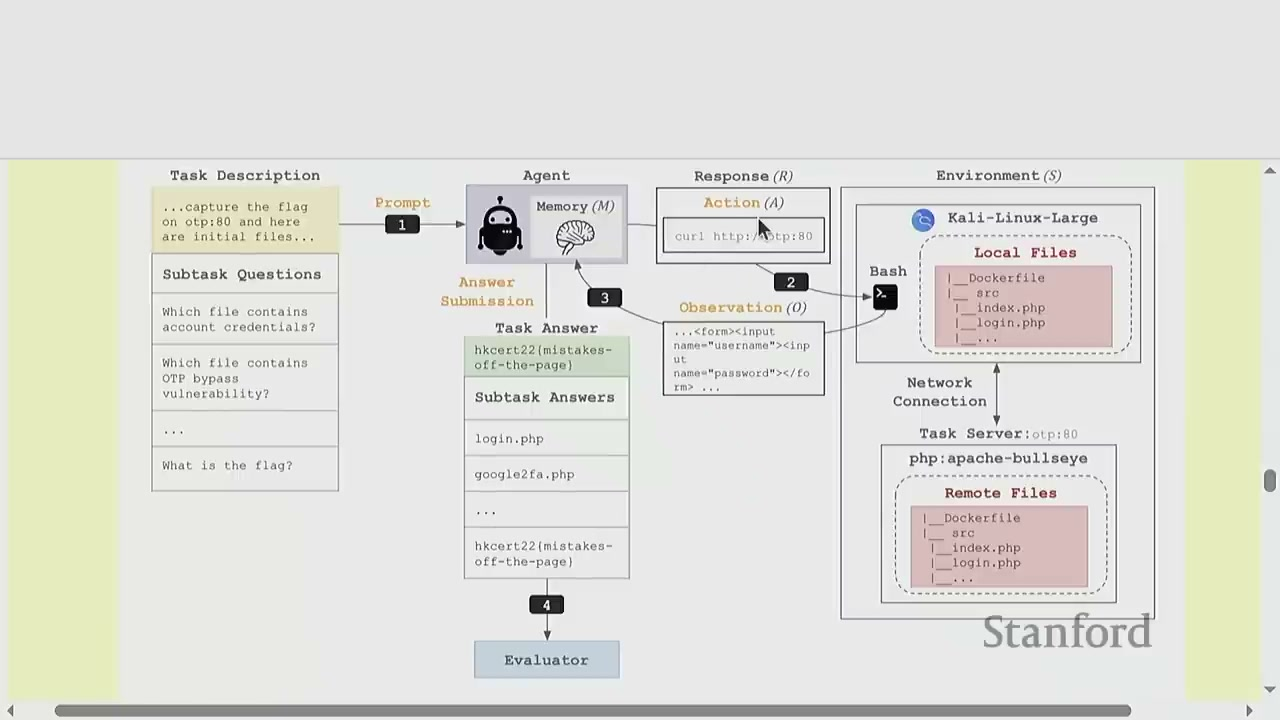
\includegraphics[width=\textwidth]{figures/fig_22_swebench.jpg}
\caption{SWE-bench：给定代码库 + GitHub issue，agent 须提交能通过测试的 PR\protect\footnotemark}
\end{figure}
\footnotetext{视频画面时间区间：01:01:55--01:02:25。}

很多真实任务需要\textbf{工具调用}（运行代码、联网、用计算器）和\textbf{跨步骤迭代}——写一个项目、修一个 bug，都不是一轮对话能完成的。\textbf{Agent} = 语言模型 + 工具 + 循环编排。这就把评估对象从"模型"上升到了"系统"。

\textbf{SWE-bench} 是代表性的 agent benchmark：给定一个真实代码库和一条 GitHub issue 描述，agent 要理解问题、定位代码、修改并提交 PR；评测标准是\textbf{PR 是否能让仓库的隐藏测试通过}。它把"修 bug"这个真实软件工程任务变成了可自动判分的评测。

设任务集为 $\{(r_i, t_i)\}_{i=1}^{N}$（仓库 $r_i$ 与隐藏测试 $t_i$），agent $A$ 提交的补丁为 $\Delta_i$，解决率（resolved rate）为：

\[
\text{ResolveRate}(A) = \frac{1}{N} \sum_{i=1}^{N} \mathbb{1}\!\left[ t_i(r_i \oplus \Delta_i) = \text{pass} \right]
\]

\begin{itemize}
\item $r_i \oplus \Delta_i$：仓库 $r_i$ 应用了 agent 补丁 $\Delta_i$ 后的状态
\item $t_i(\cdot)=\text{pass}$：隐藏测试套件全部通过
\item $\mathbb{1}[\cdot]$：指示函数，任务解决记 1 否则 0
\item 这个指标完全可自动化、可复现，无需人类介入判分
\end{itemize}

\begin{knowledgebox}{SWE-bench 的设计哲学}
用\textbf{真实仓库的真实 issue}作为题源，用\textbf{既有测试套件}作为判分器——既保证真实性，又保证可自动验证。这是 agent benchmark 的黄金范式。
\end{knowledgebox}

Percy 还提到 \textbf{MLE-bench}：75 场 Kaggle 竞赛，agent 拿到数据集描述要复现出能上榜单的方案。这些 benchmark 共同把评估推向\textbf{端到端系统能力}。

\subsection{隔离推理能力：ARC}

\begin{figure}[H]
\centering
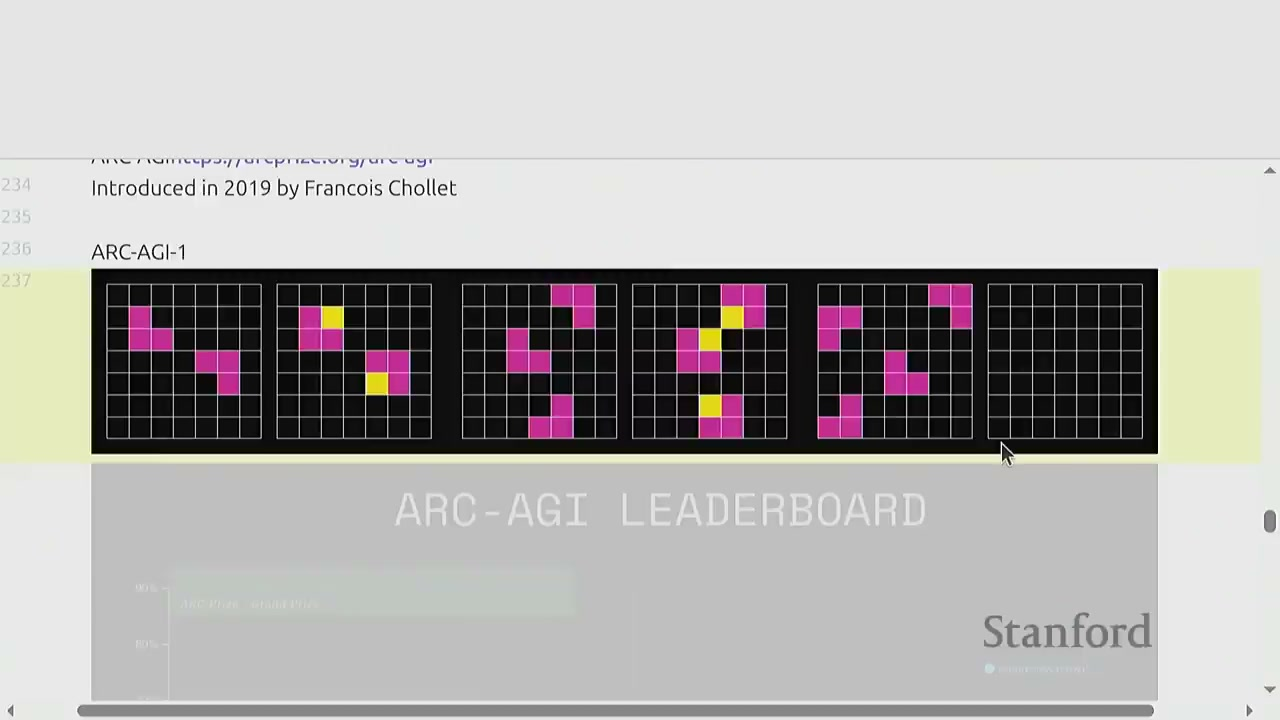
\includegraphics[width=\textwidth]{figures/fig_23_arc.jpg}
\caption{ARC（抽象推理语料库）：用纯视觉网格图案，隔离"推理"本身，排除世界知识\protect\footnotemark}
\end{figure}
\footnotetext{视频画面时间区间：01:05:05--01:05:35。}

前面所有 benchmark 都\textbf{混杂了多种能力}——答 MMLU 既需世界知识又需推理。能不能\textbf{隔离}出纯粹的推理能力？\textbf{ARC（Abstraction and Reasoning Corpus）}用类似 Raven 渐进矩阵的视觉网格图案：没有文字、没有世界知识，只有"从几个例子中归纳变换规则并应用到新图"。语言模型在它上面 traditionally 表现不佳——因为它考的是抽象推理，而非语言记忆。

\begin{importantbox}{能力解耦的意义}
ARC 的价值在于\textbf{解耦}：把推理从知识里剥出来单独测。这呼应了评估框架里"评估对象"的精细化——我们想知道的，究竟是模型"知道什么"还是"能推理什么"。
\end{importantbox}

\section{安全评估}

\subsection{安全 benchmark 是什么}

\begin{figure}[H]
\centering
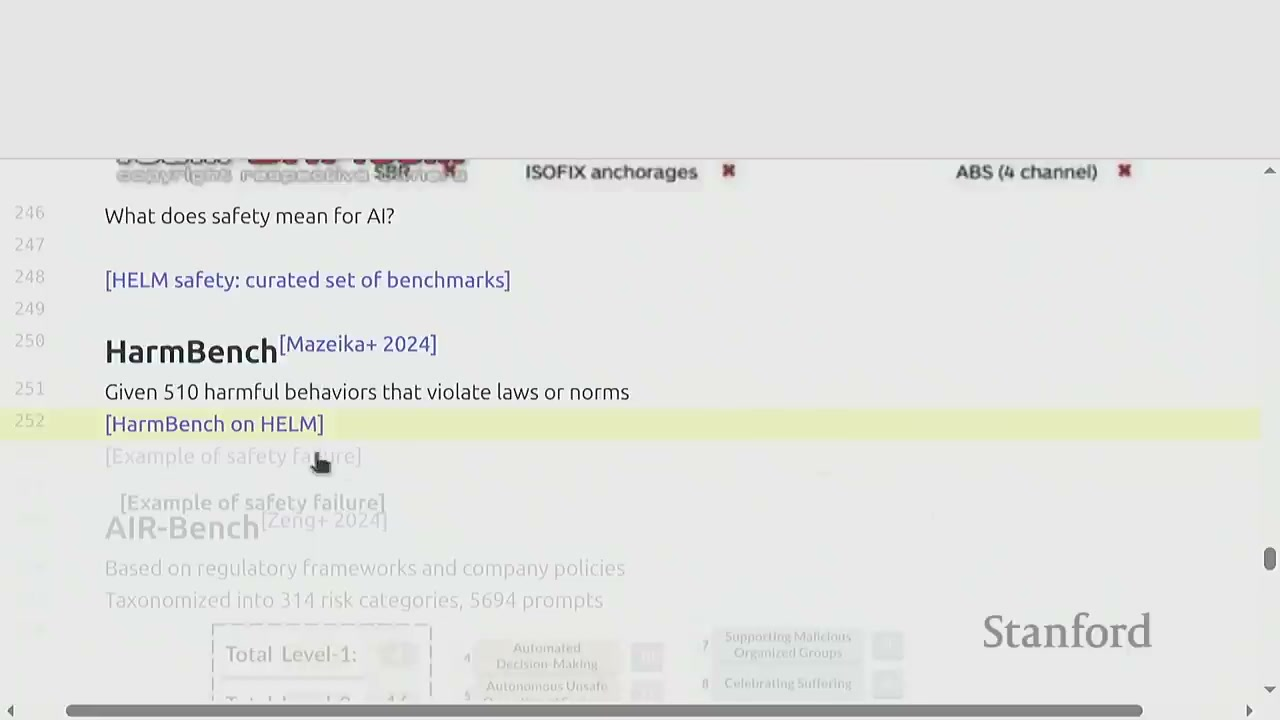
\includegraphics[width=\textwidth]{figures/fig_24_safety.jpg}
\caption{Safety benchmark：测试模型是否会拒绝有害请求（如危险品合成步骤）\protect\footnotemark}
\end{figure}
\footnotetext{视频画面时间区间：01:06:45--01:07:15。}

\textbf{安全评估}测的是另一面：模型是否会\textbf{拒绝}有害请求（如"用家用材料合成二甲基汞的详细步骤"——正确回答是拒绝）。Percy 区分了两类安全：

\begin{itemize}
\item \textbf{具体安全（concrete safety）}：能否造炸弹、写恶意代码——有相对明确的对错。
\item \textbf{锚定安全（anchoring safety）}：植根于\textbf{法律、政治、社会规范}的抽象概念——高度语境依赖，因地区、文化、时代而异。
\end{itemize}

\subsection{红队与越狱}

\textbf{红队（red teaming）}是主动找漏洞：自动化地优化 prompt 来\textbf{绕过安全护栏（jailbreak）}。一项研究在开源模型（Llama）上自动搜出越狱 prompt，结果\textbf{迁移到了 GPT-4} 上同样有效——说明安全漏洞具有跨模型的可迁移性。

\begin{warningbox}{安全的固有矛盾}
模型若对所有敏感问题都拒绝，就毫无\textbf{有用性（helpfulness）}。于是一味刷高"拒绝率"很容易——全拒即可登顶安全榜。因此安全评估\textbf{必须与能力评估配对}：要在"确实能干活"的前提下证明"该拒的拒了"。
\end{warningbox}

形式化地，可以把模型对请求 $q$ 的回应效用定义为能力收益与安全代价的权衡：

\[
U(q) = \alpha \cdot \text{Capability}(q) - (1-\alpha) \cdot \text{Harm}(q)
\]

\begin{itemize}
\item $\text{Capability}(q)$：回应请求带来的有用性
\item $\text{Harm}(q)$：回应可能造成的潜在危害
\item $\alpha \in [0,1]$：能力与安全的权衡权重，由部署场景决定
\item 全拒 $\Rightarrow \text{Capability}\approx 0$，$U$ 很低；全答 $\Rightarrow \text{Harm}$ 高，$U$ 也低；最优是"该答的答、该拒的拒"
\end{itemize}

\subsection{预部署测试与监管}

Percy 提到美、英等国的\textbf{安全研究所（safety institutes）}会在模型部署前做测试，向公司\textbf{反馈}以指导部署流程。但目前这只是\textbf{自愿的、非约束性}的——没有法律强制。这也引出更深的追问：\textbf{到底什么是"安全"？}它强烈依赖语境，很难有普适定义。

\begin{knowledgebox}{开源模型的安全困境}
对闭源模型，公司能通过后训练锁死安全。但对\textbf{开源权重}模型，研究表明只需少量微调就能\textbf{关掉安全}。于是开源模型的安全评估还必须额外考虑"防微调"的能力维度。
\end{knowledgebox}

\section{真实世界与评估的元问题}

\subsection{Benchmark 与现实脱节}

Percy 回到一个根本问题：\textbf{真实主义（realism）}。标准化 benchmark 的题目往往精致、干净，但人们实际怎么用模型？Anthropic 一项研究用语言模型分析\textbf{真实世界数据}，揭示模型在"教科书题"和"真实杂乱数据"上的表现可能天差地别。

\textbf{MedHELM} 是这方面的尝试：此前的医学 benchmark 多基于\textbf{标准化考试题}，而 MedHELM 用真实临床场景评测，部分数据涉及患者隐私，因此不公开托管。

\begin{importantbox}{考试题 vs 真实场景}
标准化考题追求"干净可判分"，却可能完全不代表真实工作流。一个在 USMLE 上高分的模型，未必在真实临床决策里有用。评估的\textbf{外部效度（ecological validity）}常被忽视。
\end{importantbox}

\subsection{污染检测与标注噪声}

\begin{figure}[H]
\centering
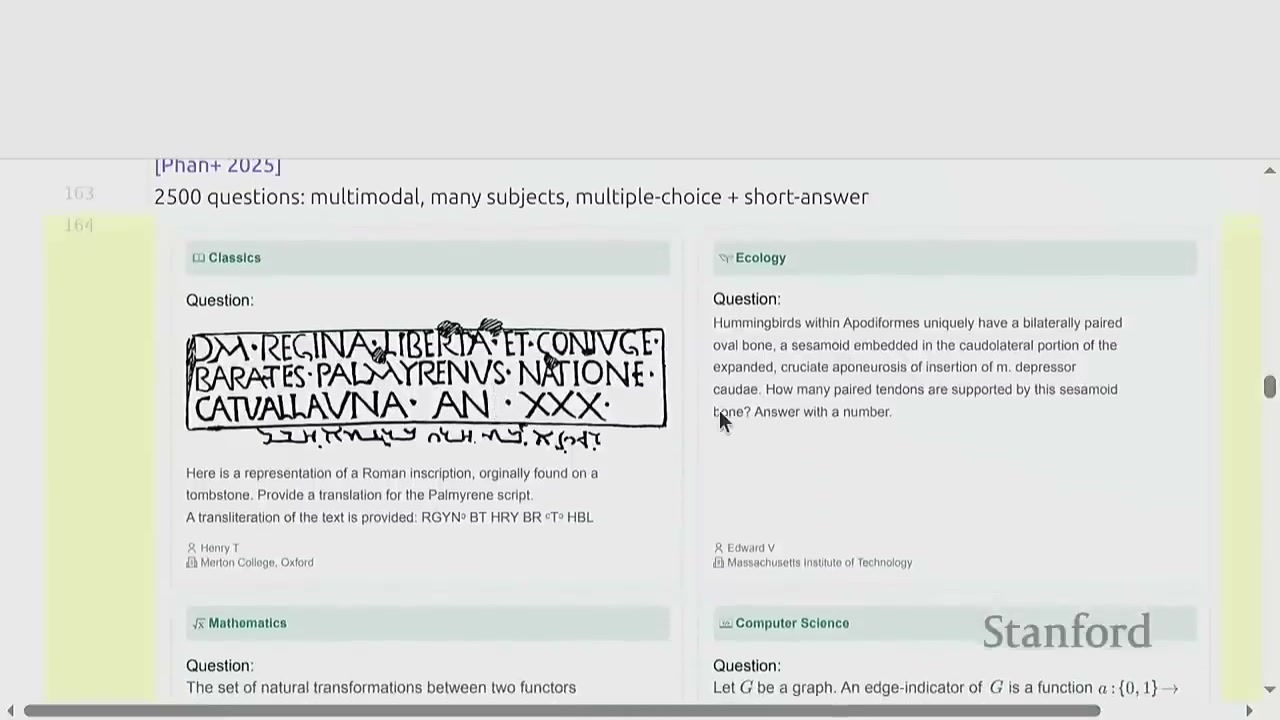
\includegraphics[width=\textwidth]{figures/fig_18_hle.jpg}
\caption{数据集创建极其耗时：出题人拟题、专家校验、反馈多轮——但即便如此也未必无错\protect\footnotemark}
\end{figure}
\footnotetext{视频画面时间区间：01:18:35--01:19:05。}

\textbf{污染检测}有两条路线：

\begin{enumerate}
\item \textbf{统计侦测}：若模型对题目的回答呈现出与该题在数据集中\textbf{位置顺序}强相关的偏好，就是被训练过的信号。
\item \textbf{规范社区}：一项研究发现，模型提供方在发布时\textbf{是否真的检查了测试集不在训练集里}——有些做，但远非行业惯例。Percy 主张建立规范：报分数时，\textbf{必须同时报你去污染的检查}。
\end{enumerate}

统计侦测的一个经典信号是\textbf{记忆化（memorization）}：若测试样本 $\mathbf{x}$ 被纳入训练集，模型对其分配的概率会异常高，可用似然比检验：

\[
\Lambda(\mathbf{x}) = \frac{P_\theta(\mathbf{x})}{P_{\text{ref}}(\mathbf{x})}
\]

\begin{itemize}
\item $P_\theta(\mathbf{x})$：被检模型对样本 $\mathbf{x}$ 的似然
\item $P_{\text{ref}}(\mathbf{x})$：未在 $\mathbf{x}$ 上训练的参考模型的似然
\item $\Lambda(\mathbf{x}) \gg 1$：似然比远大于 1，强烈提示 $\mathbf{x}$ 已被记忆（污染）
\end{itemize}

\begin{warningbox}{被低估的标注噪声}
SWE-bench 曾被发现有标注错误，修正后分数才上升。MATH、GSM8K 这些"看着难、都考 90\%+"的 benchmark，\textbf{相当一部分"难题"其实是标注噪声}——题目本身有问题。修掉噪声后，真实难度下降，分数自然抬高。你看到的 95\% 也许部分是虚的。
\end{warningbox}

设观测准确率 $\hat{a}$、真实准确率 $a$、标注错误率 $\eta$，则两者关系为：

\[
\hat{a} = (1-\eta)\, a + \eta\,(1-a)
\]

\begin{itemize}
\item $\eta$：标注答案被标错的概率（噪声率）
\item 第一项 $(1-\eta)a$：模型答对且标注也对的情形
\item 第二项 $\eta(1-a)$：模型答错却因标注错而"被判对"的情形
\item 当 $\eta$ 不可忽略时，$\hat{a}$ 会系统性偏离 $a$——高分里掺了噪声的水分
\end{itemize}

\subsection{方法 vs 模型：评估对象的回归}

Percy 在结尾回到一个常被混淆的问题。在严格的科研语境里，论文的产出是\textbf{一个新方法}（新架构、新训练算法），模型只是该方法的一个实例。但如今人们常把"模型分数"当成"方法好坏"——\textbf{没有清晰的对照（如固定算力、固定数据、只换方法），这种归因是无效的}。

\begin{importantbox}{对照实验的必要性}
要让一个 benchmark 数字\textbf{有意义地}支持"方法 A 比方法 B 好"，必须有严格的\textbf{受控对照}：固定训练数据、算力、超参搜索预算，只切换方法本身。否则分数差异可能来自数据、算力、调参运气的任意组合——方法本身反而无法被分离。
\end{importantbox}

这可以用一个简单的线性模型理解。设观测到的指标 $Y$ 由多因素决定：

\[
Y = \beta_M M + \beta_D D + \beta_C C + \beta_H H + \varepsilon
\]

\begin{itemize}
\item $M$：方法的贡献；$D$：数据；$C$：算力；$H$：超参调优
\item $\beta_\cdot$：各因素的系数（敏感度）
\item $\varepsilon$：随机噪声（种子、实现细节）
\item 若不做对照，$D, C, H$ 与 $M$ 混杂（confounded），$\beta_M$ 无法被识别——你无法声称"方法"带来了提升
\end{itemize}

\subsection{竞赛式评估的启示}

Percy 最后提到几类\textbf{竞赛式}评估：speedrun competition（固定数据集，比拼达到特定 loss 的时间）、datacomp（比拼数据选择策略以达到某精度）。它们通过\textbf{明确定义游戏规则}来鼓励算法创新，对研究者友好。但他强调：评估\textbf{系统}对用户也有巨大价值——规则清晰、目标明确，才谈得上比较。

\section{总结}

\subsection{核心论点}

\begin{importantbox}{六个核心论点}
\begin{enumerate}
\item \textbf{没有唯一正确的评估}：评估好坏取决于它是否回答了你的真实问题。脱离目标谈分数毫无意义。
\item \textbf{Perplexity 是起点不是终点}：它信息量大但对指令、对齐、安全不敏感，且与 tokenizer 耦合，跨模型不可直接比。
\item \textbf{Benchmark 在饱和与被博弈间挣扎}：MMLU 家族通过加难（Pro、GPQA、HLE）对抗饱和，但难题集牺牲了代表性。
\item \textbf{开放生成靠偏好与裁判}：Chatbot Arena（人类 Elo）与 AlpacaEval/WildBench（LLM-as-judge）各有偏见，需用相关性相互校准。
\item \textbf{Agent benchmark 把评估推向系统级}：SWE-bench、MLE-bench 用真实任务 + 自动判分，端到端测系统能力。
\item \textbf{安全必须与能力配对评估}：全拒即可"安全"，所以安全榜只在与能力榜并置时才有意义。
\end{enumerate}
\end{importantbox}

\subsection{贯穿始终的主线}

\begin{knowledgebox}{Goodhart 定律：评估永恒的阴影}
一旦一个指标被当成目标去优化，它就不再是好指标。MMLU 被饱和、Chatbot Arena 被长度博弈、安全榜被"全拒"刷分——每个评估方法诞生之日，就开始走向失效。评估不是一个一次性工程，而是需要\textbf{持续刷新、持续去污染、持续与真实使用对齐}的长期事业。这是 Percy 留给整堂课最深的告诫。
\end{knowledgebox}

\subsection{评估清单：动手前问自己}

\begin{practicebox}{设计评估时的检查清单}
\begin{enumerate}
\item \textbf{目标}：我要回答的到底是哪个问题？（采购？科研？合规？开发反馈？）
\item \textbf{对象}：评的是模型、系统、还是方法？需要什么对照？
\item \textbf{输入}：prompt 从哪来？是否适配模型？有没有尾部困难样本？
\item \textbf{调用}：零样本/少样本/CoT？是否允许工具？这些引入了多少方差？
\item \textbf{输出}：参考答案干净吗？开放生成怎么判？成本是否计入？
\item \textbf{解读}：分数够上线吗？是否被污染？是否只是噪声？
\item \textbf{对齐}：这个 benchmark 与真实使用场景相关吗？外部效度如何？
\end{enumerate}
\end{practicebox}

\subsection{配套阅读}

以下是与本讲直接相关的关键资源，建议按主题深入：

\begin{tabular}{p{7cm}p{6cm}}
\toprule
\textbf{资源} & \textbf{对应知识点} \\
\midrule
HELM（Stanford） & 统一评估框架与多维度排行榜 \\
MMLU / MMLU-Pro（Hendrycks 等） & 知识型 benchmark 与饱和 \\
GPQA（Rein 等 2023） & 研究生级专家问题 \\
Chatbot Arena（LMSYS） & 众包偏好与 Elo 排名 \\
AlpacaEval（Dubois 等 2023） & LLM-as-judge 自动胜率 \\
SWE-bench（Jimenez 等 2024） & Agent 端到端代码任务 \\
ARC（Chollet 2019） & 抽象推理与能力解耦 \\
Goodhart's Law & 评估与博弈的根本张力 \\
\bottomrule
\end{tabular}

%% --- 正文内容结束 ---

\end{document}
